\documentclass[a4paper, 12pt]{article}
\usepackage[english]{babel}
\usepackage{mathptmx}
\usepackage{fullpage}
\usepackage{graphicx}
\usepackage{siunitx}
\usepackage{textcomp}
\usepackage{listings}
\usepackage{courier}
\usepackage{framed}
\usepackage{float}
\usepackage{booktabs}
\usepackage{enumitem}
\usepackage{hyperref}
\usepackage{subcaption}
\usepackage{fancyhdr}
\setlength{\headheight}{1cm}
\usepackage{multicol}
\usepackage{apacite}
\usepackage{enumitem}
\usepackage{setspace}
\usepackage{amsmath}
\usepackage{titlesec}
\usepackage[toc,page]{appendix}
\usepackage{tabularx}
\usepackage{todonotes}
\usepackage[square,numbers]{natbib}
\setcitestyle{numbers}
\bibliographystyle{ieeetr}

\usepackage{color}
\definecolor{mygreen}{RGB}{28,172,0} % color values Red, Green, Blue
\definecolor{mylilas}{RGB}{170,55,241}
\lstset{language=R,%
    basicstyle={\ttfamily\footnotesize},
    breaklines=true,%
    stringstyle=\color{mylilas},
    commentstyle=\color{mygreen},%
    showstringspaces=false,%without this there will be a symbol in the places where there is a space
    numbers=left,%
    numberstyle={\ttfamily\tiny},% size of the numbers
    numbersep=9pt, % this defines how far the numbers are from the text
}

\titlespacing{\section}{0pt}{0pt}{-\parskip}
\titlespacing{\subsection}{0pt}{0pt}{-\parskip}
\titlespacing{\subsubsection}{0pt}{0pt}{-\parskip}

\setlist{nosep}
\usepackage[headsep=1cm, top=3cm, bottom=2.5cm, left=2.5cm, right=2.5cm]{geometry}

\title{Bayesian Modelling of the Wairakei Geothermal Surface Network}
\author{Logan Wu}

\setlength{\parskip}{\baselineskip}
\makeatletter
\fancyhead{}
\fancyhead[L]{\@title}
\fancyhead[R]{\@author}
\newlength{\drop}

\begin{document}
\begin{titlepage}
    \drop=0.1\textheight
    \centering
    \vspace*{\baselineskip}
    \rule{\textwidth}{1.6pt}\vspace*{-\baselineskip}\vspace*{2pt}
    \rule{\textwidth}{0.4pt}\\[\baselineskip]
    {\LARGE\@title}\\[0.2\baselineskip]%
    \rule{\textwidth}{0.4pt}\vspace*{-\baselineskip}\vspace{3.2pt}
    \rule{\textwidth}{1.6pt}\\[\baselineskip]
    \vspace*{2\baselineskip}
    {\Large\scshape \@author\par}
    {\itshape
    UPI: LWU308\\
    ID: 254620375}\\
    {\scshape
    Partner: Vida Fox\\
    Supervisors: Dr. David Dempsey and Dr. Cameron Walker\par}
    \vspace*{2\baselineskip}
    {\large\scshape The University of Auckland}\\
    {\itshape Department of Engineering Science}\\
    {\itshape \today}
    
\vfill
\textnormal{
\begin{abstract}
The Wairakei geothermal field is one of the oldest geothermal electricity producers in the world, and is unique in its utilisation of lower enthalpy fluids. The current operator, Contact Energy Ltd., uses a system of spreadsheets, test results and real-time measurements to update forecasts of the network and make decisions. Their model has no formal measure of uncertainty.\\
We implement a Bayesian network model that performs a statistical simulation of the Wairakei surface network, simultaneously incorporating data from multiple sources and over a long period of time to estimate the network parameters.\\
Our simulation incorporates time into production curves using a linear model, and propagates uncertainty from the wells further down the network to probabilistically verify flows where operational constraints may need to be adhered to. We also find that manual well test data and automatically logged data differ in utility, with test data being better for estimating well production parameters, and logs from the PI system being more effective for forecasting. By implementing Bayesian statistics, this system gives the field operator a systematic, numerical interpretation for the uncertainty in the network model.
\end{abstract}
}
\vfill
\end{titlepage}
\makeatother

\newpage
\pagenumbering{gobble}
\section*{Declaration}
I declare that this report is my own work except where cited. The project pair shared meetings and raw data, and this work was carried out independently of the other student in the project.

\section*{Acknowledgements}
I would like to thank both of my supervisors, Dr. David Dempsey and Dr. Cameron Walker, for not taking on any other Part IV projects and selflessly devoting all their time to ours.

\newpage
\pagenumbering{gobble}

\begin{multicols}{2}
\begin{spacing}{0}
\setcounter{tocdepth}{2}
\tableofcontents
\end{spacing}
\end{multicols}

\newpage
\pagenumbering{arabic}
\setcounter{page}{1}
\pagestyle{fancy}

%%%%%%%%%%%%%%%%%%%%%%%%%%%%%%%%%
\section{Introduction}

\begin{figure}
\centering
\begin{minipage}[t]{.48\textwidth}
  \centering
  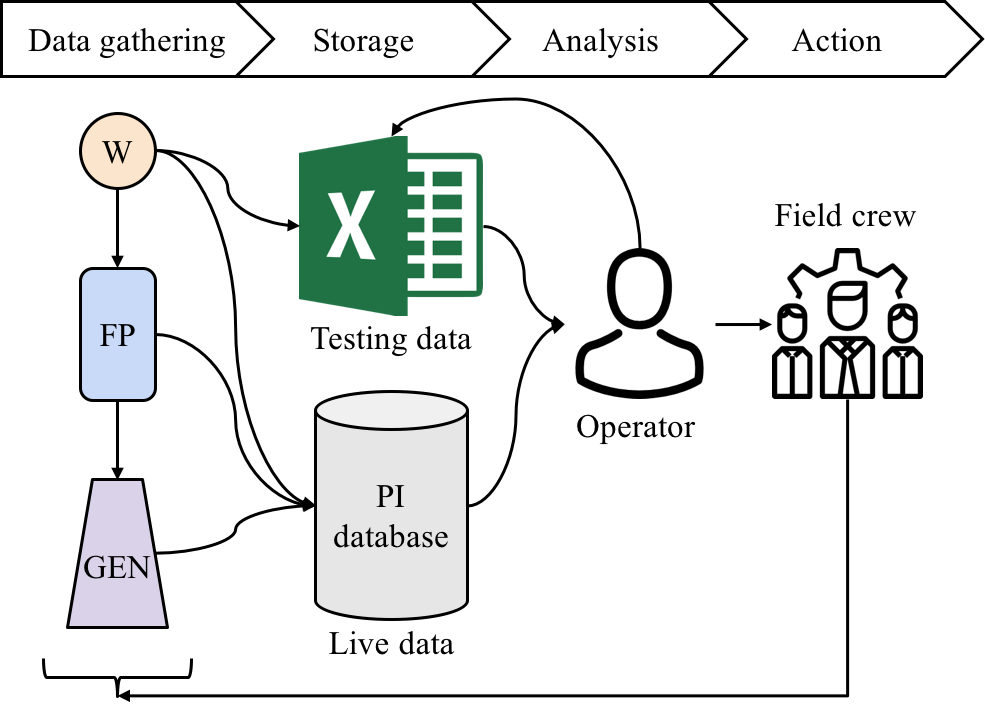
\includegraphics[width=\linewidth]{media/current_system}
  \captionof{figure}{Current system. Data on the surface network components (wells, flash plants and generators) is stored in two systems, which an operator reconciles to build a model.}
  \label{fig:current_system}
\end{minipage}\hfill
\begin{minipage}[t]{.48\textwidth}
  \centering
  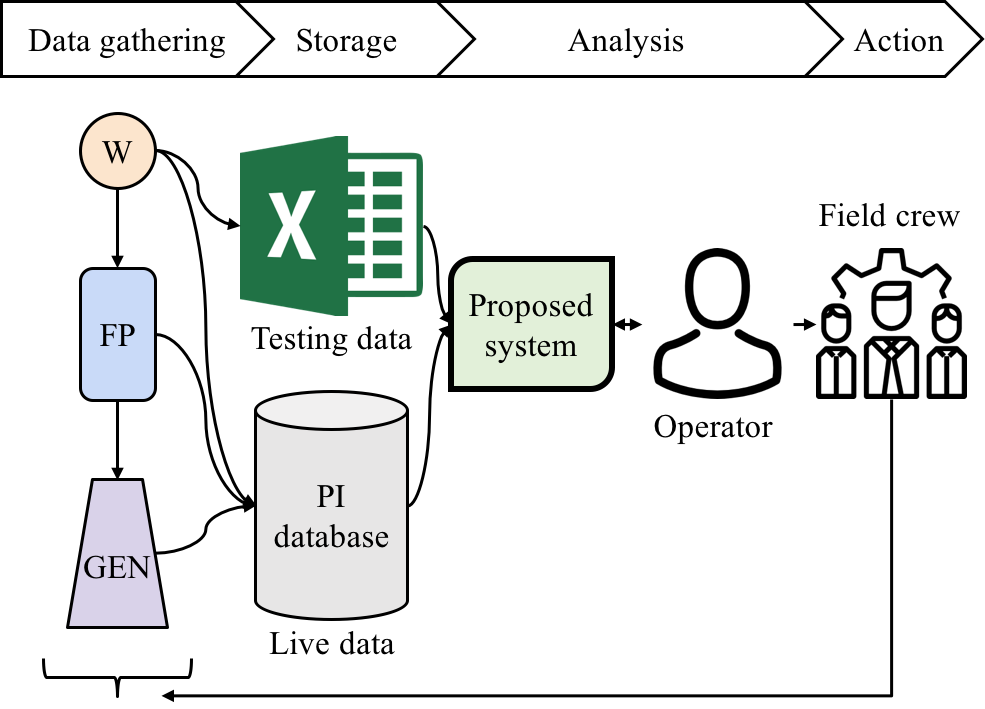
\includegraphics[width=\linewidth]{media/proposed_system}
  \captionof{figure}{Proposed system, which ingests data from both sources, incorporates it into a model and interacts with the operator to test scenarios and make predictions.}
  \label{fig:proposed_system}
\end{minipage}
\end{figure}

Contact Energy Ltd. (CEL), the operator of the Wairakei geothermal field, records a combination of field tests and live data to monitor the state of the geothermal surface network. Staff use the data to make operational decisions about well maintenance, valve positions and long-term sustainability. Currently, the flow of information in this system looks like Figure \ref{fig:current_system}. Data from flow meters and well tests is stored for analysis by an operator, who manages the maintenance and operation of the field. 

One of the major pain points is between the storage and analysis stages. To access the PI database, the operator exports data into an Excel spreadsheet. They then compare it with the well test data stored in another spreadsheet.

After calibrating the test data, running regressions and making forecasts, they obtain metrics about each well's condition and make recommendations such as whether to perform a work-over to remove deposits inside the well bore. Accessing and processing the data is a manual task, and the spreadsheets have become cumbersome and slow to open. Calibration requires experience to know what the values should look like, adding dependence on a single operator.

In this project, we develop the intermediate system shown in Figure \ref{fig:proposed_system} between the data storage and operator, that integrates the two datasets and assists in the operator's tasks by automating the statistical analysis. We also experiment with different model formulations to approximate the well production curves and demonstrate possible use cases for the results of our model.

There are two advantages to our proposed system compared with the current workflow:
\begin{enumerate}
\item Data from multiple sources are combined into a statistical model that includes uncertainty using Bayesian statistics.
\item The operator can interact with the internal model through Excel to conduct scenario analysis and automatically visualise the results.
\end{enumerate}

%%%%%%%%%%%%%%%%%%%%%%%%%%%%%%%%%
\section{Advantage of Bayesian Estimation}
Estimation of uncertainty is an essential part of drawing informative, yet realistic inferences. The current geothermal model used by CEL is deterministic. It does not take  measurement and parameter uncertainty into account when modelling the surface network of wells, pipes, flash plants and power plants. Therefore, there is a lack of understanding around how reliable the forecasts generated by the model are, and how this reliability might change in different parts of the surface network. We can use a Bayesian network model to include uncertainty in the estimates.

The barrier to Bayesian statistics has historically been the computational cost of iterative solution methods. In frequentist statistics, approximations with closed-form solutions are used. Many problems with Normal distributions have analytic solutions and are therefore cheap. An example is ordinary least-squares regression, which uses the Central Limit Theorem where the average of many residuals converges to a Normal distribution and can be characterised by just two parameters. With Bayesian statistics, no such assumptions are made. There are often no closed-form solutions, but advances in computational power have made iterative sampling methods practical.

The key components of Bayesian statistics are three functions: a prior distribution, a likelihood function and a posterior distribution. The prior $f(\theta)$ is an expert/modeller's initial belief of what the model parameters could be, before seeing any data. The likelihood function $f(x|\theta)$ is the statistical likelihood of observing the data given any parameter value drawn from the prior, and this is used to update the prior to create the posterior $f(\theta|x)$, the probability of the parameter values given both the expert knowledge and the observed data. We wish to compute the posterior for our network model, which includes deterministic and/or stochastic operations at nodal facilities such as wells, flash plants and generators.

The proportional Bayes formula to compute the posterior is:
\begin{equation}
f(\theta|x) \propto f(x|\theta)f(\theta)
\end{equation}
The use of a prior (absent in Frequentist statistics) allows the modeller to add contextual knowledge into the model. For example:

\begin{enumerate}
\item If it is known that $\theta_i \in [0,1]$, a Beta prior would be appropriate as it is non-zero on the interval $[0, 1]$. 
\item If a mass flow resides in some ballpark due to expert knowledge, a Normal distribution may be chosen, with a variance determined by the expert's certainty.
\item Or, if there is no expert knowledge, this is often represented by a uniform prior $f(\theta)\propto 1$, where any real value is equally likely.
\end{enumerate}

Am example used in our model is measurement uncertainty, with CEL estimating that power conversion factors have an error of up to 10\%. Therefore, we set a prior on multiplicative error $f(\epsilon)$ as $\text{Unif}(0.9,1.1)$. This is the preferred method because by adding extra information (assuming the prior is not misleading), we increase the bias and decrease the variance of the posterior. We refer to bias as a preference of the model towards certain values -- this is desirable as long as the bias comes from a credible source because it reduces the amount of data needed to reach the same conclusion.

The result of our analysis, the posterior distribution $f(\theta|x)$, represents our belief of the true network parameters after both specifying any expert information and observing the data. Posteriors are easily assessed as either density plots (plotting $f(\theta|x)$ by $\theta$) or 95\% credible intervals. Posterior credible intervals are also interpreted more intuitively than Frequentist confidence intervals, as our belief of a parameter value rather than a long-run average over infinite sampling. We use the term `credible interval' whenever the Bayesian interpretation is used (e.g. parameter estimates), and `confidence interval' for Frequentist interpretations (e.g. the T-test). Other differences in interpretation are detailed in Table \ref{tab:ci}.

\begin{table}
\centering
\begin{tabularx}{0.85\linewidth}{rXX}
\hline
 & Frequentist & Bayesian \\ 
  \hline
Parameter $\theta$ & Fixed by a null hypothesis $h_0$ & Unknown and probabilistic \\\hline
Data $\vec{x}$ & Random; we observe a sample & Fixed; from an unknown distribution \\\hline
95\% CI & Under repeated sampling, 95\% of confidence intervals will contain the true $\theta$ & $\theta$ has a 95\% chance of lying within the credible interval  \\
   \hline
\end{tabularx}
\caption{Differences in interpretation between the two main statistical paradigms. The Bayesian interpretation is usually more intuitive, but often the end results are similar.}
\label{tab:ci}
\end{table}

By applying computational Bayesian techniques to the Wairakei geothermal surface network, we develop a  method to fit a model to data observations, simulate probabilistic flows in the network using the posterior and incorporate uncertainty in our predictions.

%%%%%%%%%%%%%%%%%%%%%%%%%%%%%%%%%
\section{Wairakei Network Structure}

At a single point in time, the Wairakei surface network can be represented as a directed, acyclic graph shown in Figure \ref{fig:network_diagram}. There are three types of nodes: wells, flash plants and generators. Each node has inputs, transformations,  outputs and associated parameters that we can estimate. As some wells have multiple flash plants they can be routed to, the active arcs are pre-determined according to the configuration we wish to simulate.

\begin{figure}
  \centering
  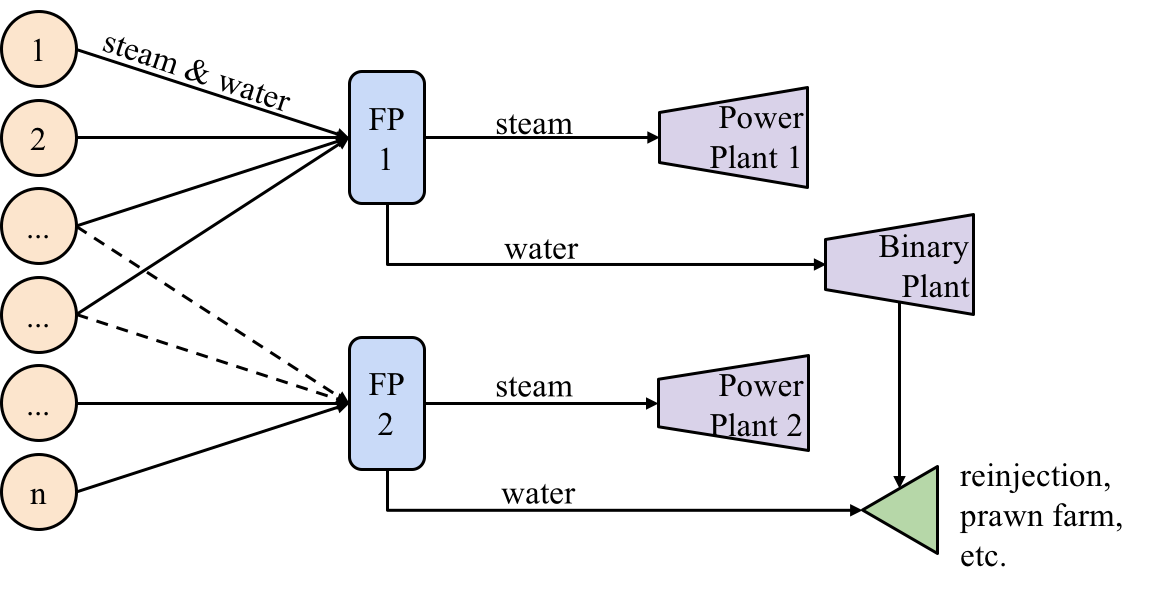
\includegraphics[width=0.5\linewidth]{media/network_diagram}
  \captionof{figure}{Simplified structure of the Wairakei geothermal surface network. Some wells can send steam to a selection of flash plants, but only one at a time (the solid/dashed lines).}
  \label{fig:network_diagram}
\end{figure}

\subsection{Well Nodes}
In the model, each well begins with an operating well-head pressure selected by the operator or set to the most recent measurement. Wells generate mixed-phase fluid with an enthalpy $h_i$ and mass flow rate $\dot{m}_i$. Well-head pressure is the pressure measured at the gauge, so zero indicates the well is venting into the atmosphere at maximum flow, and maximum pressure means the well is shut with no flow.

The relationship between mass flow and well-head pressure can be predicted using wellbore simulators such as TOUGH2, but these take a long time to run and it is easier for CEL to evaluate an statistical approximation as $\dot{m} = f(\theta)$. CEL approximates $f$ using well test data, using three data points from a given day to fit two degrees of freedom. Often the full data set includes many sets of tests over several years.

CEL fits multiple models using a small subset of the data for each set of well tests. We use their data set to calibrate a regression model predicting mass flow with time effects and uncertainty by using data over different dates and from multiple sources. By incorporating more data, our regression model can also estimate uncertainty in its parameters.
%\todo{Introduce equations}

\subsection{Flash Plant Nodes}
Flash plants take flow inputs from a subset of wells, such that many wells map to each flash plant. Configurations can come from historical records, external optimisation routines or any hypothetical setup we wish to test.

At a flash plant $j$, the extensive (mass-flow dependent) properties are summed over its subset of wells $I(j)$ and intensive (per unit mass-flow) properties are mass flow-weighted averages.
\begin{align} \
\dot{m}_j &= \sum_{i\in I(j)} \dot{m}_i\quad \forall j \label{eq:fp_mf} \\
h_j &= \frac{\sum_{i\in I(j)} \dot{m}_i h_i}{\sum_{i\in I(j)} \dot{m}_i} \label{eq:fp_h}
\end{align}
These formulae assume conservation of mass and enthalpy, which holds if network components are sufficiently sealed and insulated. Enthalpy loss in the Wairakei pipes is estimated at 0.6\% in the pipes by Zarrouk \cite{Zarrouk:2014}, who concludes that it is negligible.

Impure steam from the wells causes pitting and corrosion in the generator turbines. Flash plants convert the fluid into steam with one or two pressure drops to boil the liquid component of the fluid \cite{Grant:2011}. The resulting steam mass flow from a drop to pressure $P$ can be calculated by:
\begin{equation}
\dot{m}_{\text{steam},j} = \chi\dot{m}_j,\quad \chi= \min{\left\{\max{\left\{\frac{h_j - h_{f@P}}{h_{fg@P}}, 0\right\}}, 1\right\}}
\end{equation}
where $h_{f@P}$ is the specific enthalpy of saturated water at pressure $P$ and $h_{fg@P}$ is the latent heat of evaporation. Vapour quality $\chi$ is bounded between zero and one, and the remaining mass flow is the liquid fraction. At some plants there are multiple pressure drops, leading to intermediate pressure (IP) and low pressure (LP) steam.

The outflowing steam and water can go to the same or different generators. For example, several flash plants send steam and water to the Poihipi and binary plants respectively.

\subsection{Generator Nodes}
Generators accept intermediate and low pressure steam or water from flash plants, where the subset of flash plants supplying steam to generator $k$ is $I_{\text{steam}}(k)$ and the subset of flash plants supplying water is $I_{\text{water}}(k)$. The power output $\dot{W}_k$ from a generator $k$ with efficiency $\eta_k$ is proportional to the mass flow of steam feeding it:
\begin{align}
\dot{W}_k &= \eta_k \sum_{i\in I_{\text{steam}}(k)} \dot{m}_{\text{steam},i}\quad\text{for steam generators}\\
&\text{or}\nonumber\\
\dot{W}_k &= \eta_k \sum_{i\in I_{\text{water}}(k)} \dot{m}_{\text{water},i}\quad\text{for pentane (binary) generators} \label{eq:power}
\end{align}
We are interested in the posterior distribution of total power output, $\sum_{k\in K}, \dot{W}_k$, as this is what we wish to maximise. Analysis of intermediate variables within the network gives insight into where sources of variation or uncertainty in total power output arise.

%%%%%%%%%%%%%%%%%%%%%%%%%%%%%%%%%
\section{Data Sources}
We use data supplied by Contact in several forms, including network schematics, raw numerical data and expert knowledge about uncertainty and limits in the field. We wish to build a production curve model and use this to make forecasts, given the operating pressures for each well. A component of this project is integrating multiple data sources to predict mass flow because neither of the raw data sources covers all the wells on their own.

\subsection{Network Structure}
Contact has provided a schematic indicating the connectivity of wells, to flash plants, to generators. In some cases, wells have in-built flash plants. These are treated as a single dummy flash plant where only steam enters and exits. When a well has the ability to feed to several flash plants, the configuration is pre-determined by the operator.

\subsection{Well Test Data}
Well tests from as far back as 2002 are recorded in an Excel spreadsheet. Wellbore tests are performed at multiple operating pressures to fit a production curve, as discussed in the Literature Review. The spreadsheet also contains results from tracer flow tests (TFTs), which are easier and cheaper to run because the well can remain connected to the network. We use regression techniques to replicate the production curves with more data.

Tests are only performed on the liquid wells. Well-head pressure, mass flow and enthalpy are recorded manually. The liquid wells are wells with a mixed-phase fluid output, and are the main focus of this model because of their readily available data and relationship with the flash plants that separate their wet steam.%\todo{Change (see David's comment)}
%What are you excluding and why? What data are missing/would be useful to collect? What are the implications of not having this data?
% (Note, these are topics that should be covered eventually, not necessarily in this section. However, as this is where you start to discuss the data, it may be a useful time to introduce the reader to data limitations?)
`Dry' wells (wells with integrated separators that only output steam) do not have well test data, and are covered using exported flow meter data from CEL's automatic loggers.

\subsection{PI Flow Meters}
Real-time data is supplied using flow meters. The benefit of live data is that it is stored once a day in a PI system (treated here as a generic database) in a regular time-series containing every meter. It is therefore much more regular than the well test data. The parameters recorded include well-head pressure, separator pressure and mass flows for some facilities.

%\todo{Better description of flow meter usage and time series}

Twenty liquid wells also have pressure gauges and flow meters logged in PI, and seventeen dry wells are not included in the liquid wells regression data. The data from the twenty wells shown in Figure \ref{fig:pi_data} is included in the production curve regression, and we include one month (thirty instances) of data to increase the weight in the regression on the most up-to-date points. We also use them to forecast the operating pressures. However, they cannot regress the production curve on their own because they tend to all be of the same well-head pressure and the regression parameter estimation will be ill-conditioned.

\begin{figure}
  \centering
  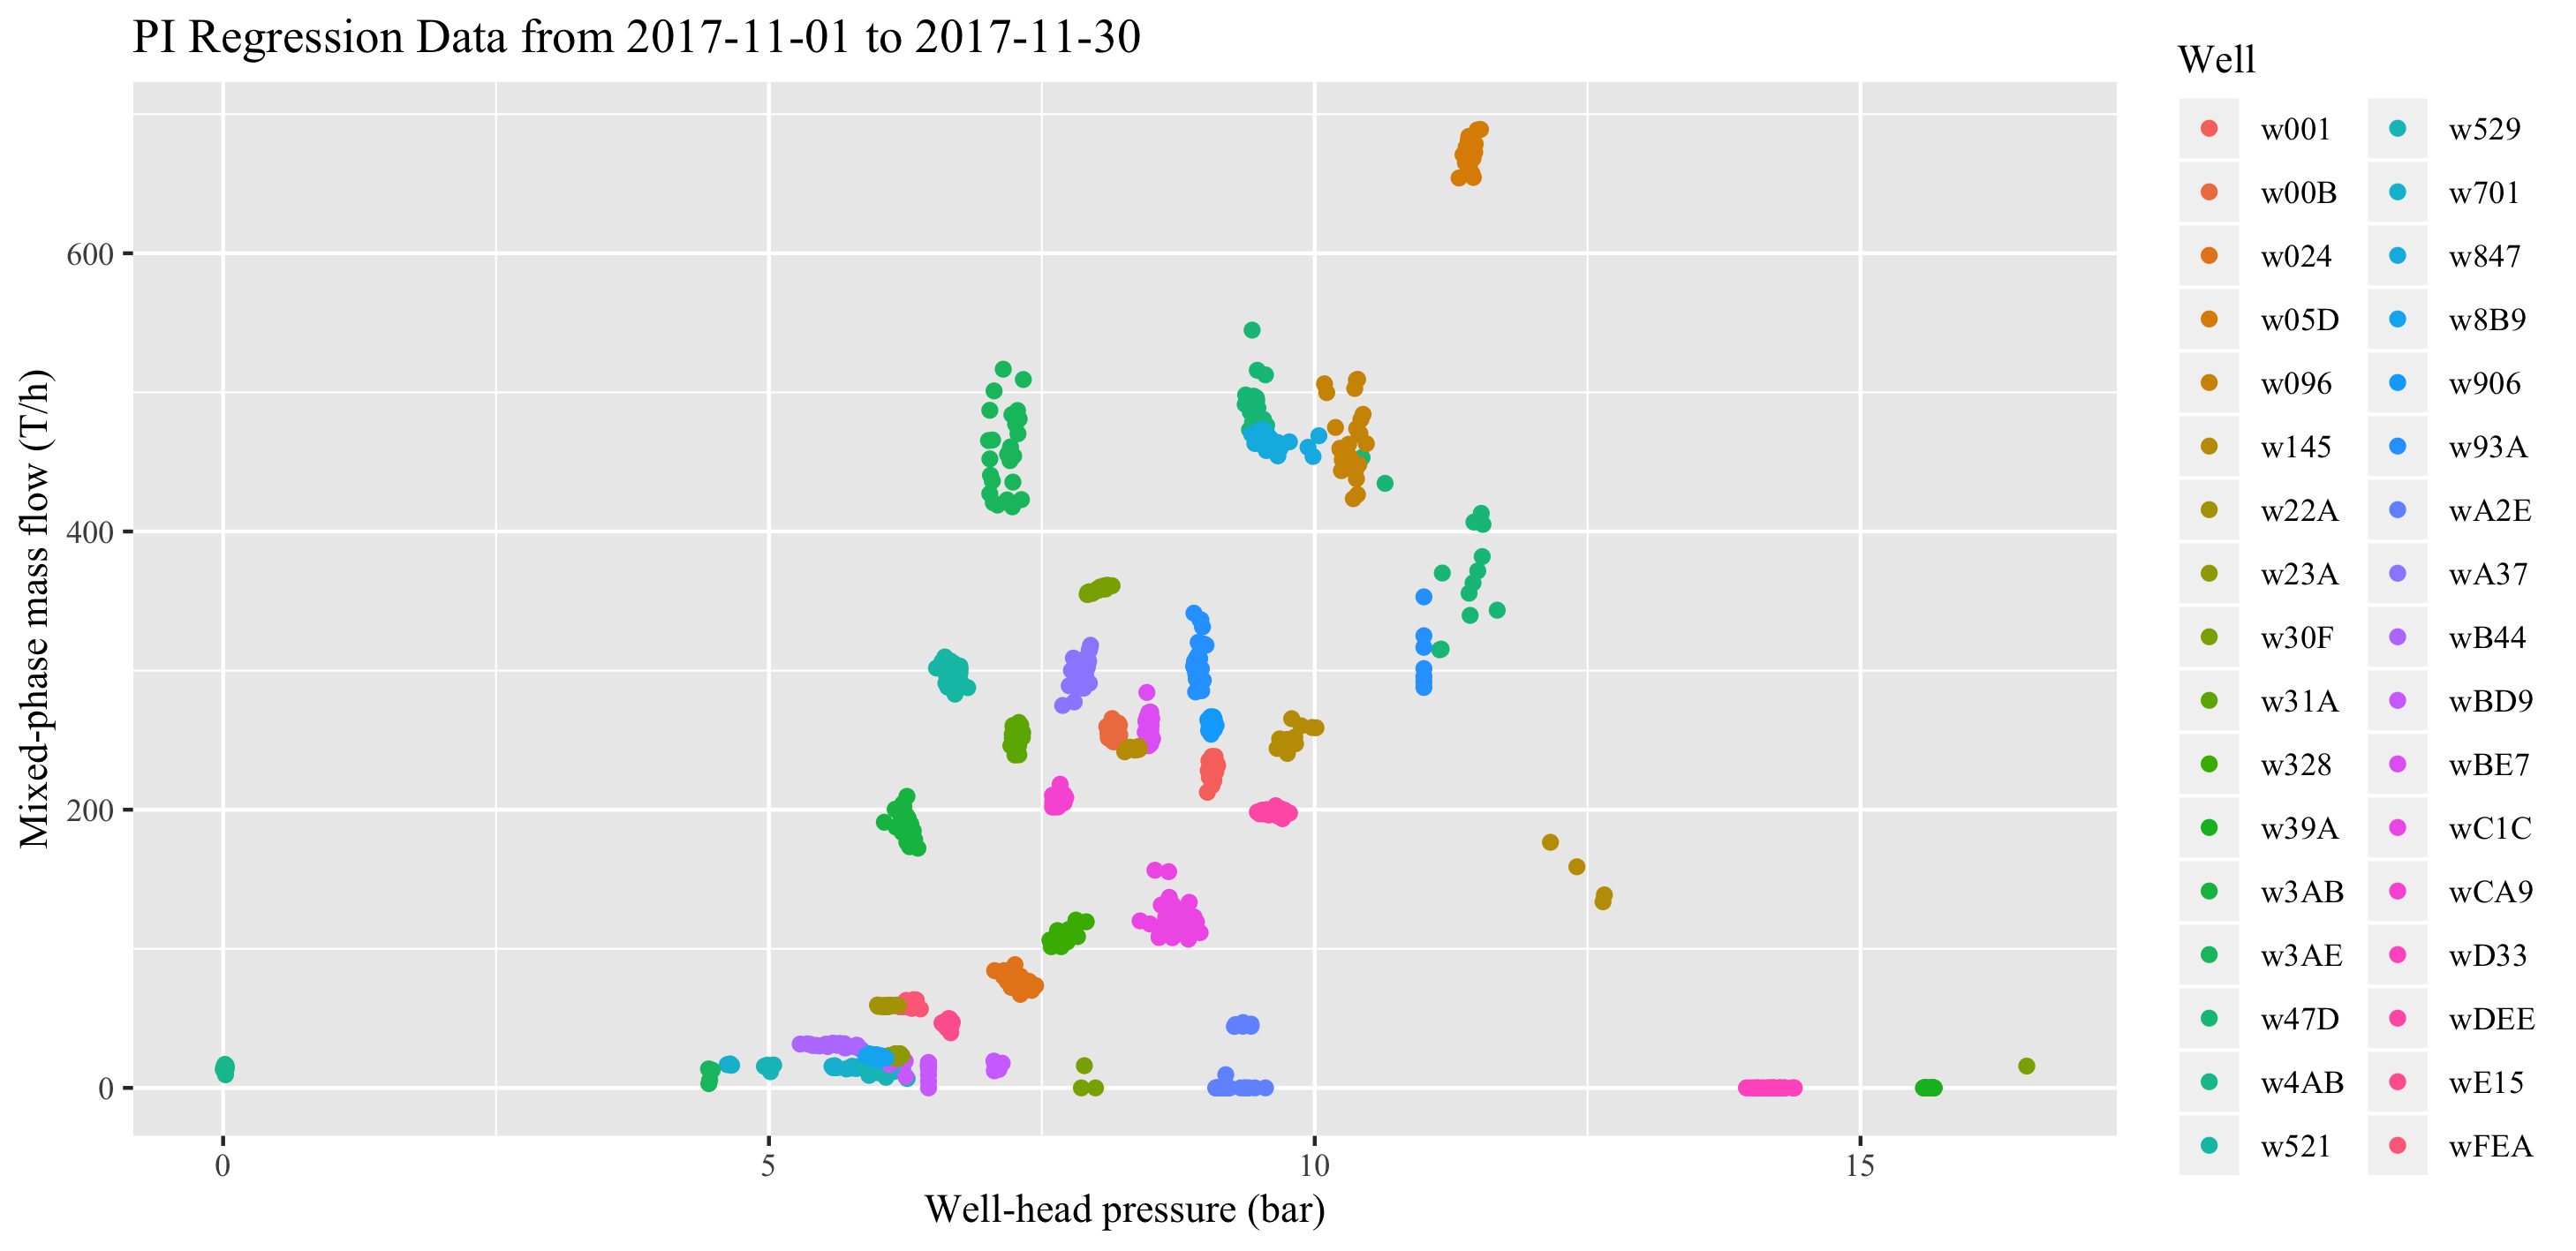
\includegraphics[width=\linewidth]{media/pi_data}
  \captionof{figure}{One month of the most recent regression data from the PI database. We use a combination of the wellbore test data (not shown) to estimate the regression parameters, and the PI data to increase the weight and precision for short-term forecasts. Note how data is tightly clustered -- this forces regressions to fit the PI data closely and is desirable if our predictive covariates are close to the PI data.}
  \label{fig:pi_data}
\end{figure}

PI data is used for the ten wells without well-head pressure in a time-series analysis without a production curve. This allows us to `fill in' the gaps from the wellbore test data even though we cannot model the relationship between well-head pressure and mass flow.

\subsection{Uncertainty}
To take full advantage of the Bayesian framework, we want to specify well-informed parameters. We have obtained prior estimates for some of the measurement uncertainties by correspondence with Contact Energy:

\begin{enumerate}
\item Well test mass flow measurements are $\pm$5\%-10\%
\item Flash plant mass flow measurements are $\pm$10\%
\item Steam to power conversion factors are up to $\pm$5\%
\end{enumerate}

Turning these statements into prior specifications is at the modeller's discretion and will be discussed for the model. However, in practice most sensible priors work if there is enough data available.

\subsection{Constraint Limits}
Flash plants have a flow limit on the fluid components. This data is not a component of the Bayesian model, but can be used when analysing the outputs to check the probability of a constraint violation given a certain network configuration.
% fp24        fp62        fp28  
% "fp14"      "fp15"      "fp16" 
\begin{enumerate}
\item fp24 $<$ 525 T/h of IP and LP steam
\item fp62 $<$ 775 T/h
\item fp28 IP $<$ 420 T/h
\item fp28 IP+ $<$ 450 T/h. These two limits are added together for IP and LP steam.
\end{enumerate}

%%%%%%%%%%%%%%%%%%%%%%%%%%%%%%%%%
\section{Data Integration}

\begin{figure}
  \centering
  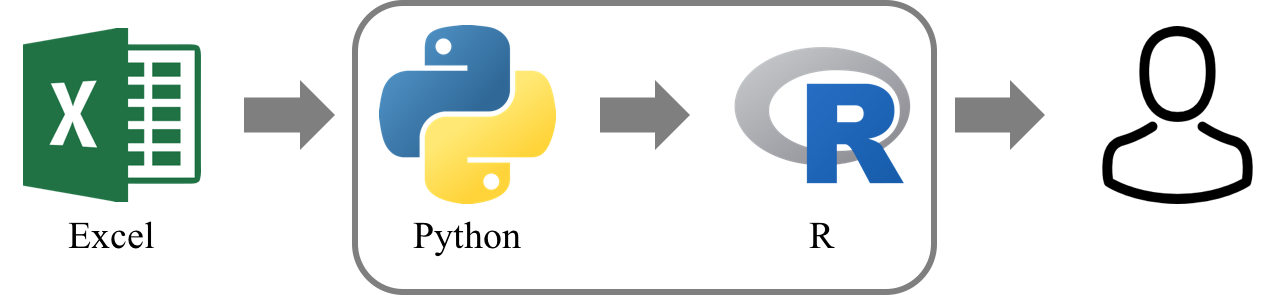
\includegraphics[width=0.5\linewidth]{media/workflow}
  \captionof{figure}{Our project includes a Python script to process the sample data files, and an R script which runs a model and processes the results.}
  \label{fig:workflow}
\end{figure}

Direct integration of our routine with Contact's PI systems was not possible for this study because of the sensitivity of live asset data. Exported Excel worksheets therefore provide the main source of data input for our implementation. This section details how we extract the raw data from provided Excel samples, how we process it and what processed data our statistical analysis requires.

\subsection{Data Extraction}
Accessing the data using the Microsoft Excel desktop application is slow, on the order of ten minutes for the sample data supplied, but much longer for the actual operational spreadsheet. Therefore, we use a Python script that accepts our unmodified data spreadsheets and immediately converts the data into efficient data frame objects. Without the overhead of Excel and the myriad of formulae within the spreadsheet, loading the data into memory from storage takes seconds.

Our Python routine implements sufficient automatic data-cleaning capabilities that fix known inconsistencies such as capitalisation, reject incomplete or erroneous lines, and discriminate between data and meta-data such as comments. Data cleaning takes negligible time.

\subsection{Pre-Processing}
The original Excel spreadsheets are in human-readable formats. They include well names rather than well IDs, and lack certain metadata such as the quantities of each facility or the mappings of wells to flash plants.

The second half of the Python script maps facility names to unique integer IDs and converts time formats into the number of days since an arbitrary baseline. These allow the data to be ingested by R. We hash all the well and flash plant names before generating outputs. Wells begin with ``W" and flash plants begin with ``FP".

We found 75 wells with more than one data point available. Several wells had insufficient data to fit a regression with three parameters, but they were all inactive wells and did not affect the network.

\subsection{Automatic and Manual Configuration}
The rest of the workflow is carried out in R. To make the program usable to non-programmers, R reads in configuration options from a separate Excel spreadsheet. Here, the user configures the well mappings and the pressures at which they intend to operate the wells. The entire network structure can also be changed to test scenarios with different facilities.

An R script reads in the processed data and the configuration file. It uses these to construct instructions for our simulation, specifying the stochastic network's structure and parameters. R also acts as our simulation interface, performing post-processing and visualisation of the outputs.

%%%%%%%%%%%%%%%%%%%%%%%%%%%%%%%%%
\section{Simulation Methods}
When calculating a posterior density, there is a tradeoff between flexibility and efficiency, with Markov Chain Monte-Carlo (MCMC) methods being the most flexible and analytic evaluation being the most efficient but sometimes impossible. We use a specific implementation of MCMC called JAGS through RJAGS, a package for the R language. This section details the components of JAGS used by our model.

\subsection{JAGS}

\begin{figure}
  \centering
  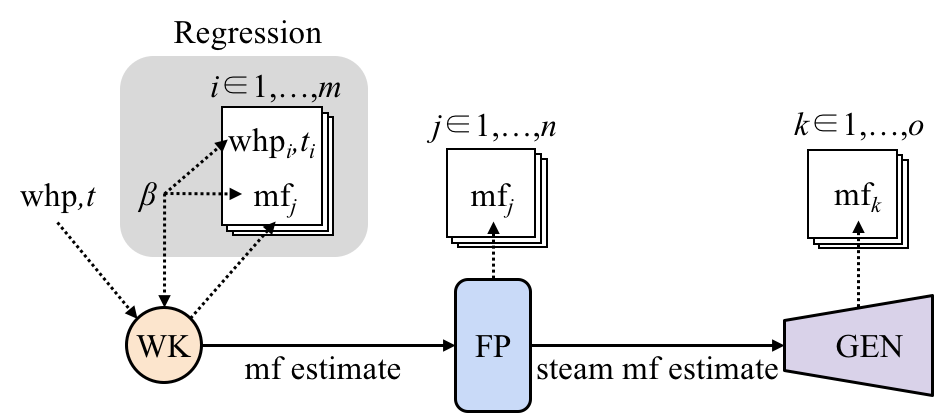
\includegraphics[width=0.5\linewidth]{media/jags_diagram}
  \captionof{figure}{A directed, acyclic graph showing the relationships between the main variables in the model. A regression is constructed at the wells, and mass flows propagate down the network to make predictions at downstream facilities.}
  \label{fig:jags_diagram}
\end{figure}

JAGS (Just Another Gibbs Sampler) is a GNU-licensed program that implements a Markov Chain Monte-Carlo method called Gibbs sampling. The exact sub-components of its Gibbs routine are abstracted as a black-box to the user through an R-like syntax.

The stochastic model we input into JAGS is structured as a a directed, acyclic graph, shown in Figure \ref{fig:jags_diagram}. Solid lines show deterministic relationships and dotted lines are stochastic relationships. To computationally evaluate a joint posterior distribution, JAGS samples from the priors $f(\theta)$ at the root nodes (here, the well-head pressures \emph{whp} and regression parameters $\beta$) and propagates forward through the arcs. When a parameter value reaches a node we observe through measurements such as mass flow, the likelihood function $f(\vec{x}|\theta)$ is computed. The product of prior and likelihood $f(\vec{x}|\theta)f(\theta)$ becomes the posterior probability $f(\theta|\vec{x})$ for the set of parameter values $\theta$ in that iteration.

By computing the joint posterior, we extract the values of the regression coefficients and estimates for flows at any point in the network.

\subsection{Sampling Algorithms}
At run-time, JAGS automatically chooses the most appropriate sampling algorithm for each node, and different nodes can use different methods. These methods come from separate modules -- \emph{base} JAGS and \emph{BUGS}.

Both of the following sampling methods are used in iterations of a Gibbs Sampler, which will be discussed in Section \ref{sec:gibbs}.

\subsubsection{BUGS::Conjugate}
The conjugate sampler in the BUGS (Bayesian inference Using Gibbs Sampling) module is used when a parameter's posterior is a conjugate distribution to the prior. Conjugate distributions are where the posterior $f(\theta|x)$ and the prior $f(\theta)$ come from the same family of distributions. This holds when the prior is the conjugate prior to the likelihood $f(x|\theta)$. The conjugate distributions (priors and posteriors) used in this model are the Normal and Gamma distributions, when the likelihood is a Normal distribution.

Conjugate priors and likelihoods are used wherever possible because the resulting posterior can be calculated analytically. For example, if we have the likelihood of a parameter as $f(\vec{x}|\mu,\sigma^2)\sim N(\mu,\sigma^2)$ where the conjugate prior distributions on mean and variance are $N(\mu_0,\sigma^2_0)$ and $\text{Inv-}\gamma(\alpha,\beta)$ respectively, we can calculate the analytic posterior for the individual parameter assuming the other is fixed:
\begin{align}
f(\mu|\vec{x},\sigma^2) &\sim N\left( \frac{1}{\frac{1}{\sigma^2} + \frac{n}{\sigma^2}} \left( \frac{\mu_0}{\sigma^2_0} + \frac{\sum\vec{x}}{\sigma^2} \right) , \left( \frac{1}{\sigma^2_0} + \frac{n}{\sigma^2} \right)^{-1} \right)\\
f(\sigma^2|\vec{x},\mu) &\sim \text{Inv-}\gamma \left( \alpha+\frac{n}{2} , \beta+\frac{\sum(\vec{x}-\mu)^2}{2} \right)
\end{align}
Note that in JAGS, the Normal distribution is often parameterised by precision $\tau = 1/\sigma^2$ rather than variance, leading to a Gamma conjugate prior instead of Inverse-Gamma.

Once the posterior parameters are obtained, samples are obtained by a range of methods often specific to one distribution family such as the Box-Muller method, an efficient method for transforming independent uniform (pseudo) random variates into standard Normal samples.

\subsubsection{base::Slice}
A Slice Sampler is a special form of random walker (Metropolis-Hastings) that is relatively simple to implement. In our model, it is used for all other parameters in the model that do not use conjugate distributions. The principle of slice sampling treats a univariate density as a uniform bivariate density, with one of the variates giving the same steady-state posterior as the original univariate \cite{Neal:2003}.

\begin{figure}
  \centering
  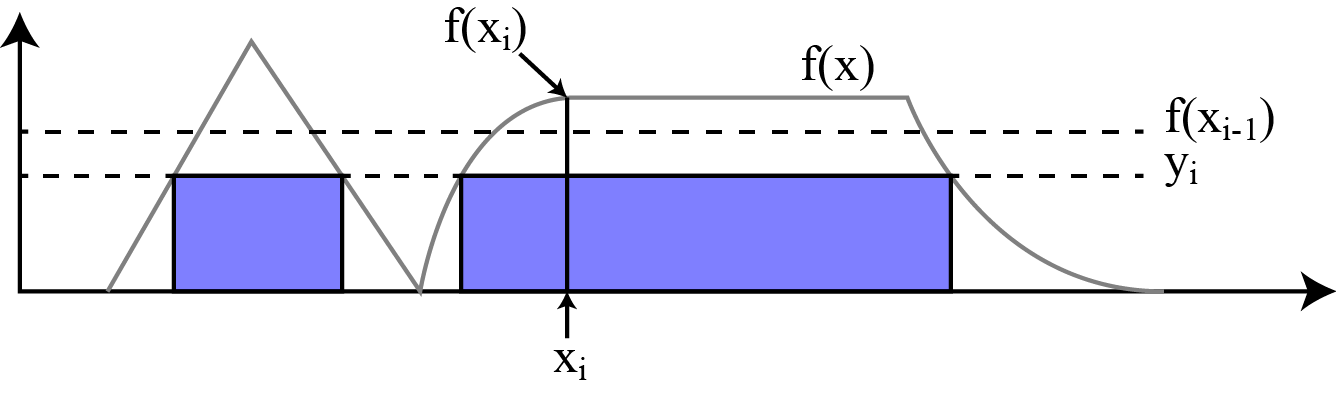
\includegraphics[width=0.5\linewidth]{media/slice_sampling}
  \captionof{figure}{A single iteration of slice sampling where a bivariate MCMC state space is constructed from a univariate density.}
  \label{fig:slice_sampling}
\end{figure}

The steps to take a slice sample are demonstrated in Figure \ref{fig:slice_sampling}:

\begin{enumerate}
\item Given $x_{i-1}$, sample $y_i$ uniformly from $[0, f(x_{i-1})]$.
\item Given $y_i$, sample $x_i$ uniformly from $\left\{ x | f(x) > y_i \right\}$.
\end{enumerate}

The long-run distribution of $x_i$ will converge on $f(x)$. Slice sampling can also be used for discrete variables, but our model only uses continuous parameters.

By solving for the set $\left\{ x | f(x) > y_i \right\}$ (not a trivial task for multimodal distributions), we allow the sampler to jump to any $x\in \left\{ x | f(x) > y_i \right\}$ and it avoids issues faced by other Metropolis algorithms where the random walker can become trapped by zero-valued regions .

\subsection{Gibbs Sampling} \label{sec:gibbs}
The previous methods are all implementable as part of a Gibbs sampling algorithm. A Gibbs sampler is a MCMC (Markov Chain Monte-Carlo) method, where each iteration depends on the state of the chain in the previous iteration in a stochastic function determined by the individual samplers.

Our goal is to evaluate the full joint distribution of all the parameters in our model, which is much more difficult than evaluating univariate or bivariate distributions. MCMC allows us to construct an ergodic Markov chain whose equilibrium or stationary distribution converges on the full, multivariate joint distribution. If it is ergodic, it will satisfy two conditions:

\begin{enumerate}
\item The chain can explore all possible parameter states from any starting state.
\item When run to infinity, its expected state distribution equal the joint distribution.
\end{enumerate}

In the Gibbs sampler, each iteration consists of sampling one parameter (or a block of parameters when possible, e.g. multivariate Gaussian) given the most recent values of the other parameters. One iteration proceeds as follows, where $i$ is the iteration for $p$ variables:
\begin{align}
\theta_1^{(i)} &\sim f\left( \theta_k|\vec{x}, \theta_2^{(i-1)}, \theta_3^{(i-1)},\dots, \theta_p^{(i-1)} \right)\\
\theta_2^{(i)} &\sim f\left( \theta_k|\vec{x}, \theta_1^{(i)}, \theta_3^{(i-1)},\dots, \theta_p^{(i-1)} \right)\\
&\vdots\nonumber\\
\theta_p^{(i)} &\sim f\left( \theta_k|\vec{x}, \theta_1^{(i)}, \theta_2^{(i)},\dots, \theta_{p-1}^{(i)} \right)
\end{align}
This specific MCMC scheme is useful because instead of sampling from a $p$-dimensional posterior, we sample from $p$ one-dimensional posteriors. Although this means each sample is not independent as would be expected from direct sampling routines, its equilibrium state still converges to the correct distribution. The time taken to reach equilibrium depends on how well the random walkers mix within their distributions, which is why conjugate and slice samplers are effective as they do not use a fixed step-size.

% The Gibbs sampler can be proven to satisfy the MCMC conditions [REF STATS 731]. JAGS uses the its constructed Markov chain with the univariate conjugate and slice sampling methods to approximate the joint posterior distribution of the geothermal surface network.

%%%%%%%%%%%%%%%%%%%%%%%%%%%%%%%%%
\section{Simulation Implementation}
JAGS code is language-agnostic and defined using a text string, Appendix \ref{sec:jagscode}. We use R instead of similar Python packages because the R interface is better supported. The RJAGS package also includes extra model and convergence diagnostics that are not available in Python, but the model declaration is still the same in any language.

There are three main steps to running a JAGS model: model specification, post-processing and model diagnostics.

\subsection{Model Specification}
JAGS code is declarative and interpreted simultaneously. Our code can still be interpreted as a set of steps where each block leads into the next, beginning at the wells and progressing through the network to the generators.

\subsubsection{Covariate Centering}
Our code contains a generalised linear model (GLM) in Equation \ref{eq:linreg} that is incompatible with JAGS' \emph{GLM} module, a specialised sampler for GLMs that is efficient when there is covariance between the parameters. Since we cannot use the module, we center the covariates. For example:
\begin{equation}
x_\text{whp} \leftarrow x_\text{whp} - \overline{x_\text{whp}}
\end{equation}
When there is high covariance, univariate samplers mix poorly because the step of one parameter is highly dependent on the value of another parameter rather than being mostly random. Centering the covariates makes the expectation of covariance zero, and we observe better mixing afterwards.

\subsubsection{Well Production Curve Regression}
One of CEL's current tasks is to fit a model to well production curves, where mass flow is a function of well-head pressure. Production curves change over time as the well and reservoir conditions change. Grant and Bixley propose a shifted elliptic form because it has interpretable real-world parameters of a maximum pressure and a maximum mass flow \cite{Grant:2011}.
\begin{equation}
\frac{\left( \dot{m}-\beta_1 \right)^2}{\beta_2^2} + \frac{P_\text{whp}^2}{\beta_3^2} = 1
\end{equation}
Contact Energy's existing spreadsheets use a centered ellipse, which only requires two data points to fit rather than three for the extra axis shift parameter:
\begin{equation}
\frac{\dot{m}^2}{\beta_1^2} + \frac{P_\text{whp}^2}{\beta_2^2} = 1
\end{equation}
Our model does not need to estimate maximum pressures and mass flows, since these are theoretical interpretations and are not observed during normal operation \cite{Marsh:2015}. Therefore, we are not restricted to this form of equation, and we can use a linear regression, which is accurate in the vicinity of the data when the production curve can be approximated as a first-order multivariable Taylor series. The Taylor series assumption holds because well tests and PI data are taken at the exact or similar well-head pressures as our predictions, and we use recent data when possible.

Elliptic models have convergence issues in Bayesian regression. A potential cause is the square root operation, which is undefined for negative arguments. If we want to use a linear, non-curved model, we must check whether curvature is present in the data. Since we cannot fit an elliptic model, we add a quadratic $P_\text{whp}^2$ term to the linear model and compare the deviance information criterion (DIC), a goodness of fit measure for Bayesian models. Raw DIC results are shown in Table \ref{tab:curvature}.

\begin{table}
\centering
\begin{tabular}{lrr}
  \hline
& Quadratic & Linear \\ 
  \hline
Mean deviance & 50423 & 51378 \\
Penalty & 3429 & 1054 \\
Penalised deviance & 53851 & 52432\\
   \hline
\end{tabular}
\caption{DIC comparison of two GLM candidates, concluding that the linear model is a better fit to the data. The DIC monitor was run for 1000 samples each.} 
\label{tab:curvature}
\end{table}

The quadratic model has a lower mean deviance because adding extra polynomial terms will always fit the data better. However, the penalty on the number of effective parameters is higher. The penalised deviances of both models are on the same order of magnitude, so the difference in fitting ability is very small. We therefore prefer the linear model for the interpretability of its parameters.

One of our extensions to the current Contact model is to incorporate time as a covariate. This allows for estimation of the production decline over time and enables forecasting for the future. The equation we fit is:
\begin{equation} \label{eq:linreg}
\dot{m} = \beta_0 + \beta_\text{whp}P_\text{whp} + \beta_\text{date}t + \epsilon,\quad \epsilon\sim N(0, \sigma^2)
\end{equation}
and the corresponding Normal likelihood function per data point (the full likelihood is the product of its components):
\begin{equation}
L\left( \dot{m} | \vec{\beta},\sigma^2,P_\text{whp},t \right) = \frac{1}{\sqrt{2\pi\sigma^2}} e^{-\frac{-\dot{m} + \beta_0 + \beta_\text{whp}P_\text{whp} + \beta_\text{date}t}{2\sigma^2}}
\end{equation}
where $\dot{m}$ is the mass flow, $P_\text{who}$ is a specified well-head pressure, $t$ is a specified number of days after a baseline, and $\epsilon$ is a Normally distributed error of unknown variance. This form has several benefits over the other models considered:

\begin{enumerate}
\item Coefficients are interpretable as rates of change, rather than theoretical maximum limits in the elliptical model.
\item A simpler model with fewer parameters is less likely to over-fit to the data.
\item There are no root or power operations. Sampling is significantly faster (~5x).
\end{enumerate}

This model assumes the trend in the relationship is linear with time, the same assumption currently made by CEL in their spreadsheets. We also assume a stationary distribution of independent errors $\sigma^2$, which are a product of measurement errors and flow variance. We derive a prior for the measurement error from CEL, and sample from flow variance when we make predictions. In cases where $P_\text{whp}$ is unavailable, such as from the PI database, we drop the $\beta_\text{whp}P_\text{whp}$ term, leading to the assumption that $P_\text{whp}$ is constant. This assumption is true as long as there is no change in back-pressure in the network from a configuration change, and the condition of the well is steady between the measurements and the time of prediction.

We sample the regression parameters to estimate $\beta_\text{date}$, the mass flow decline over time, and $\sigma^2$, flow variance.

We use a hierarchical Bayes structure to set priors on the regression coefficients $\vec{\beta},\tau=1/\sigma^2$, where $\tau$ is precision and is often used because it makes the analytic calculations simpler. Rather than making every individual parameter non-informative, we use the assumption that parameters between wells come from the same (unknown) distribution:
\begin{align}
\beta_i &\sim N\left( \mu_\beta,\tau_\beta \right)\\
\tau &\sim \gamma\left(\alpha_\tau,\beta_\tau\right)
\end{align}
where the hyper-parameters have an non-informative prior, $f\left(\mu_\beta,\tau_\beta,\alpha_\tau,\beta_\tau\right) \propto 1$.
 
This is physically motivated because:
\begin{enumerate}
\item For $\beta_\text{date}$, pressure loss in the field over time affects nearby wells.
\item For $\beta_0$ and $\beta_\text{whp}$, wells of similar types and locations should have similar production curves.
\end{enumerate}
This is not the same as saying the parameters between the wells are identical. Instead, it fits a distribution of well production curves from which each well is observed. Adding this bias gives a reduction in variance for wells with insufficient data. We instead make an educated imputation that their production curve is similar to the wells we have data for, rather than having absolutely no imputation at all.

Verification of our regression model includes plots of observed mass flows against fitted mass flows, and a residual plot using standardised residuals:
\begin{equation}
\epsilon_\text{std} = \frac{\hat{\dot{m}} - \dot{m}}{\text{sd}\left( \hat{\dot{m}} \right)}
\end{equation}
where $\hat{\dot{m}}$ is sampled from the Bayesian regression.

A well-fitting regression shows a linear correlation between the fitted and observed values. If we believe the residuals are Normally distributed, the standardised residual plot will have a constant Normal distribution across all the fitted values. We present diagnostic plots in Figure \ref{fig:diagnostics}. There is good correlation in the Observed $\sim$ Fitted plot and standardised residuals have no trend. %The residual plot also validates our implementation of errors, where the observed variance is $\sigma^2$ multiplied by a measurement error of $<$10\%. The standardised residuals become significantly inflated without this.
% CHANGE ABOVE
%\todo{Comment on residual error?}

\begin{figure}
\centering
  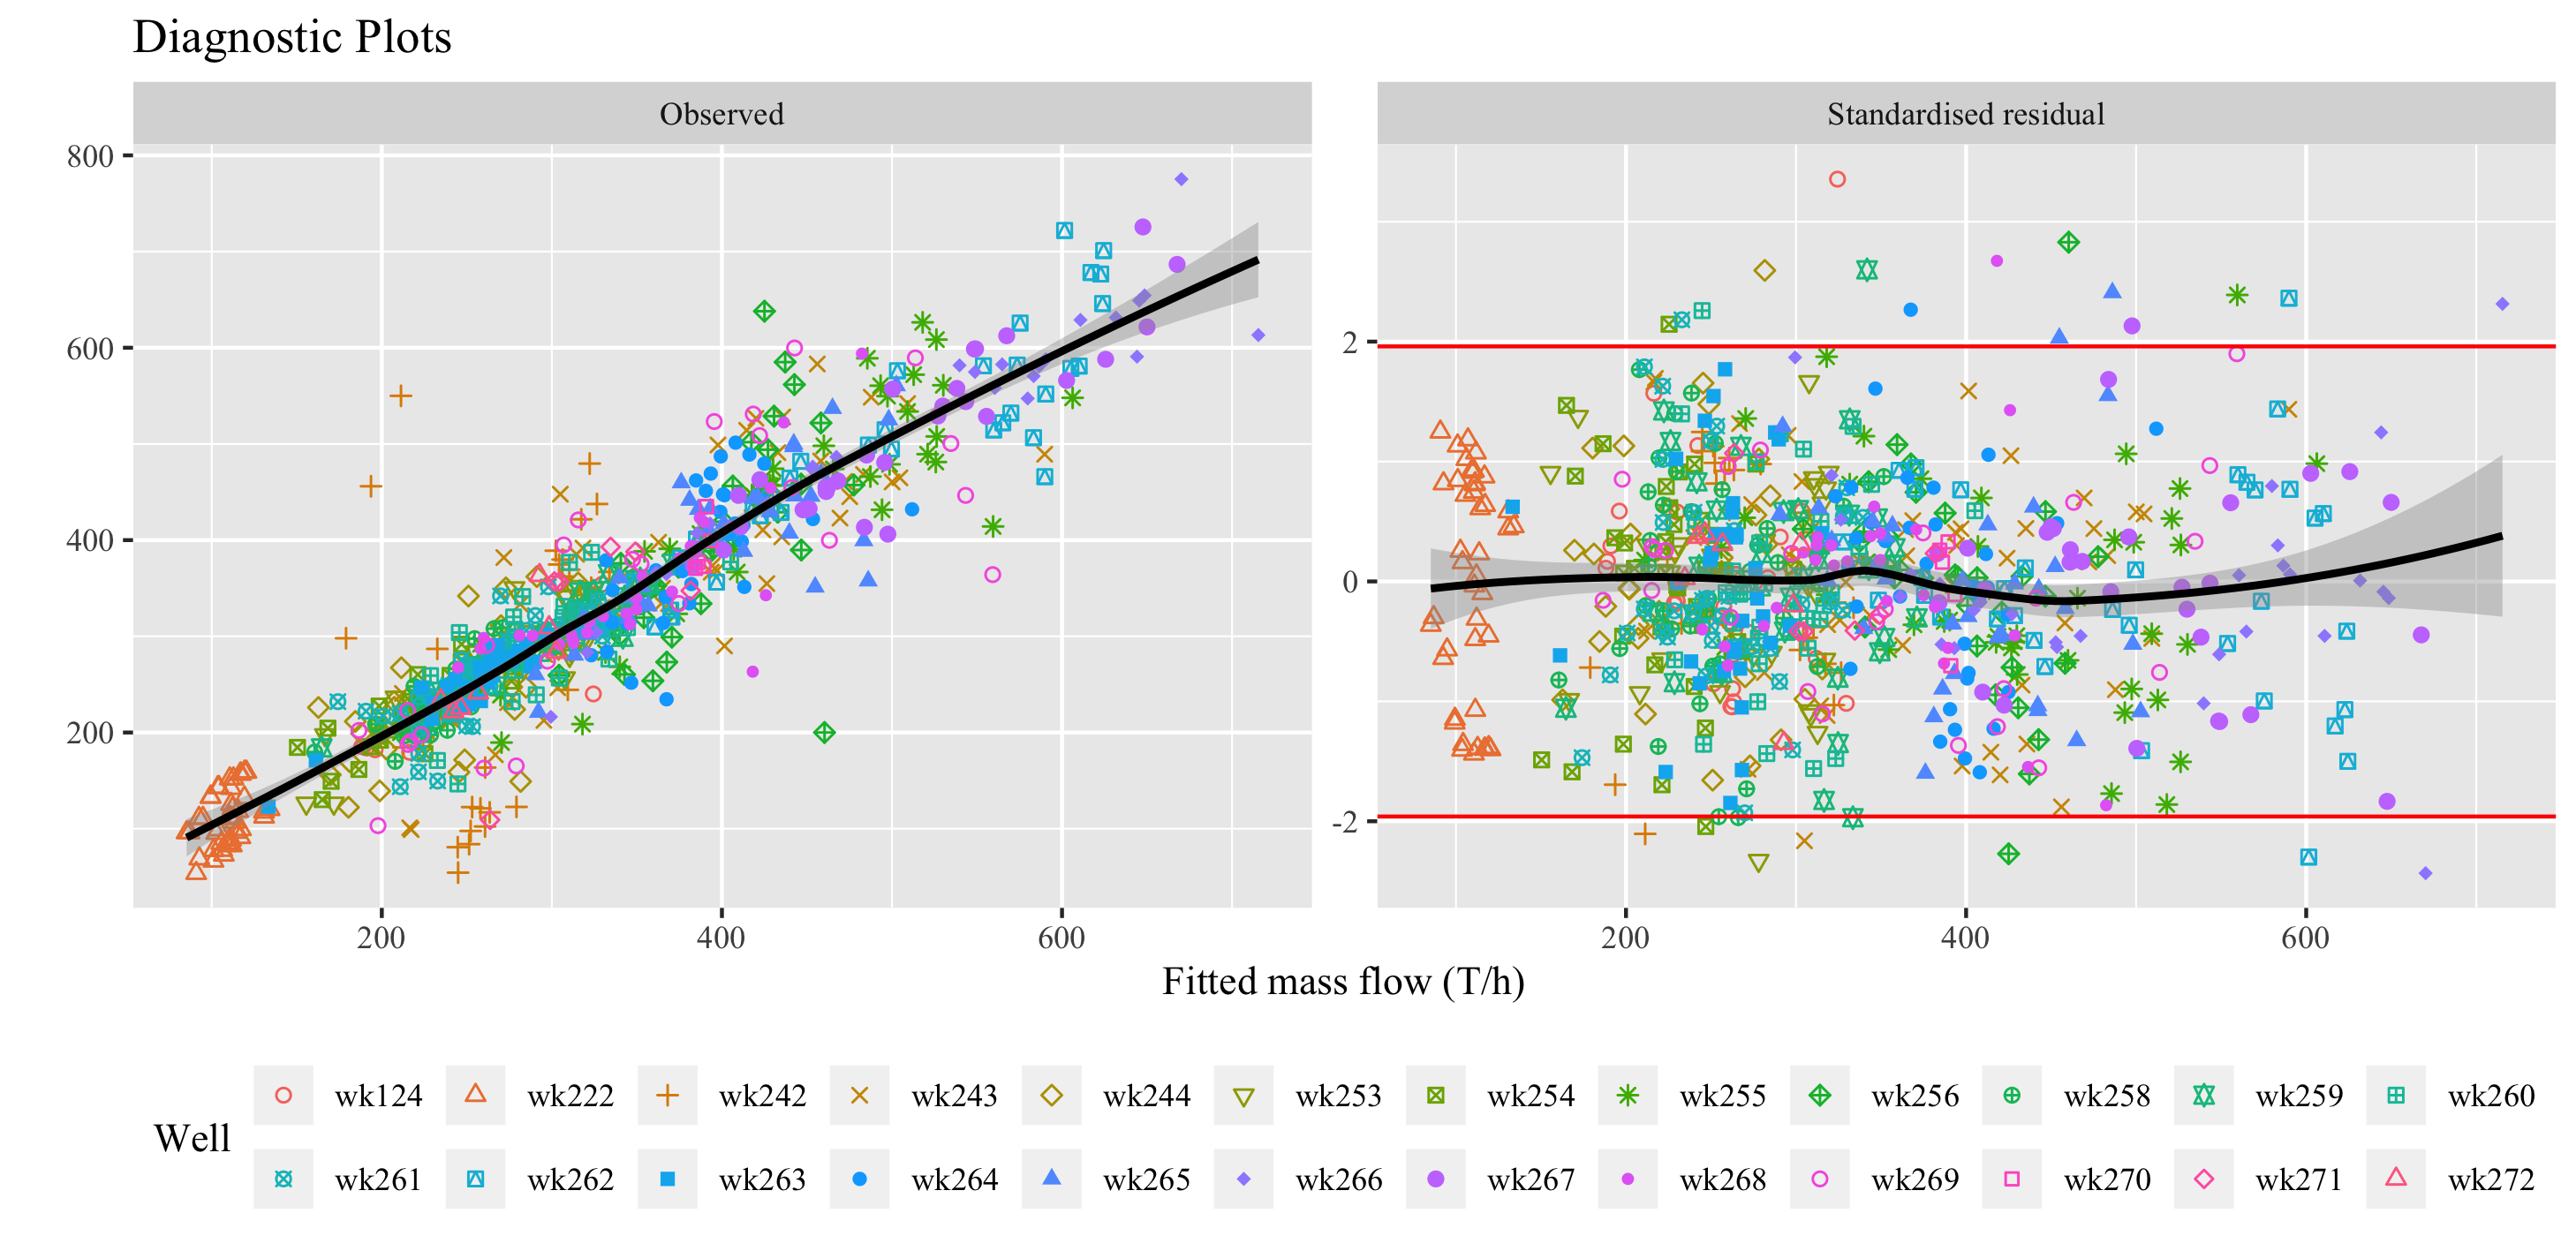
\includegraphics[width=\linewidth]{media/diagnostics}
  \captionof{figure}{Diagnostic plots with the observed response against fitted values, and residuals against fitted response. These diagnostics suggest a good fit to the data. The same diagnostic plots faceted per well are included in the appendices, figures \ref{fig:observed} and \ref{fig:stdres}, showing curvature in several wells but overall the linear fit is sufficient.}
  \label{fig:diagnostics}
\end{figure}

\subsubsection{Prediction}
With posterior production curves fitted for most wells, e.g. Figure \ref{fig:production_curve}, we can estimate the mass flows at a given well-head pressure and date, specified in the configuration file. We also assign a measured enthalpy to the well flows, or apply a hierarchical posterior to any missing enthalpy values. Wells without production curves are imputed using a time-series on the PI data -- see Figure \ref{fig:ts_experiment} for examples of the time series regression.

Figure \ref{fig:full_network} shows the modelled connectivity between wells, flash plants and generators. Dummy generators have been added so that flash plants can send one type of flow (e.g. intermediate pressure steam) to one generator, and another (e.g. water) to a second generator. This diagram is useful for showing the overall structure of the conceptual model, but can also be used to verify that the model configuration has been specified correctly in the Excel interface.

\subsubsection{Flash Plant Flows}

\begin{figure}
\centering
\begin{minipage}[t]{.48\textwidth}
  \centering
  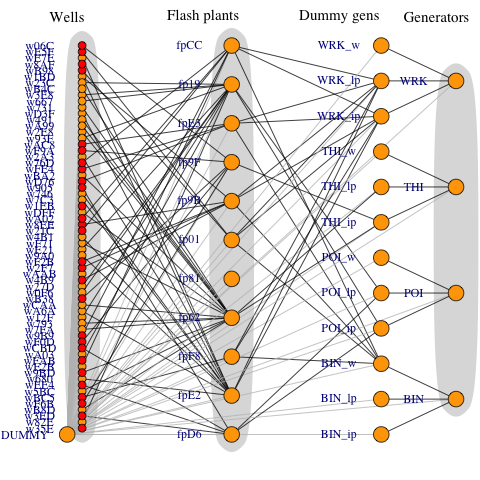
\includegraphics[width=\linewidth]{media/full_network}
  \captionof{figure}{Full network diagram, with flows from left to right. Red wells indicate forecasts have been filled in from the PI data without a production curve, and dummy arcs are in grey. Dummy arcs allow IP/LP/water to be split up.}
  \label{fig:full_network}
\end{minipage}\hfill
\begin{minipage}[t]{.48\textwidth}
  \centering
  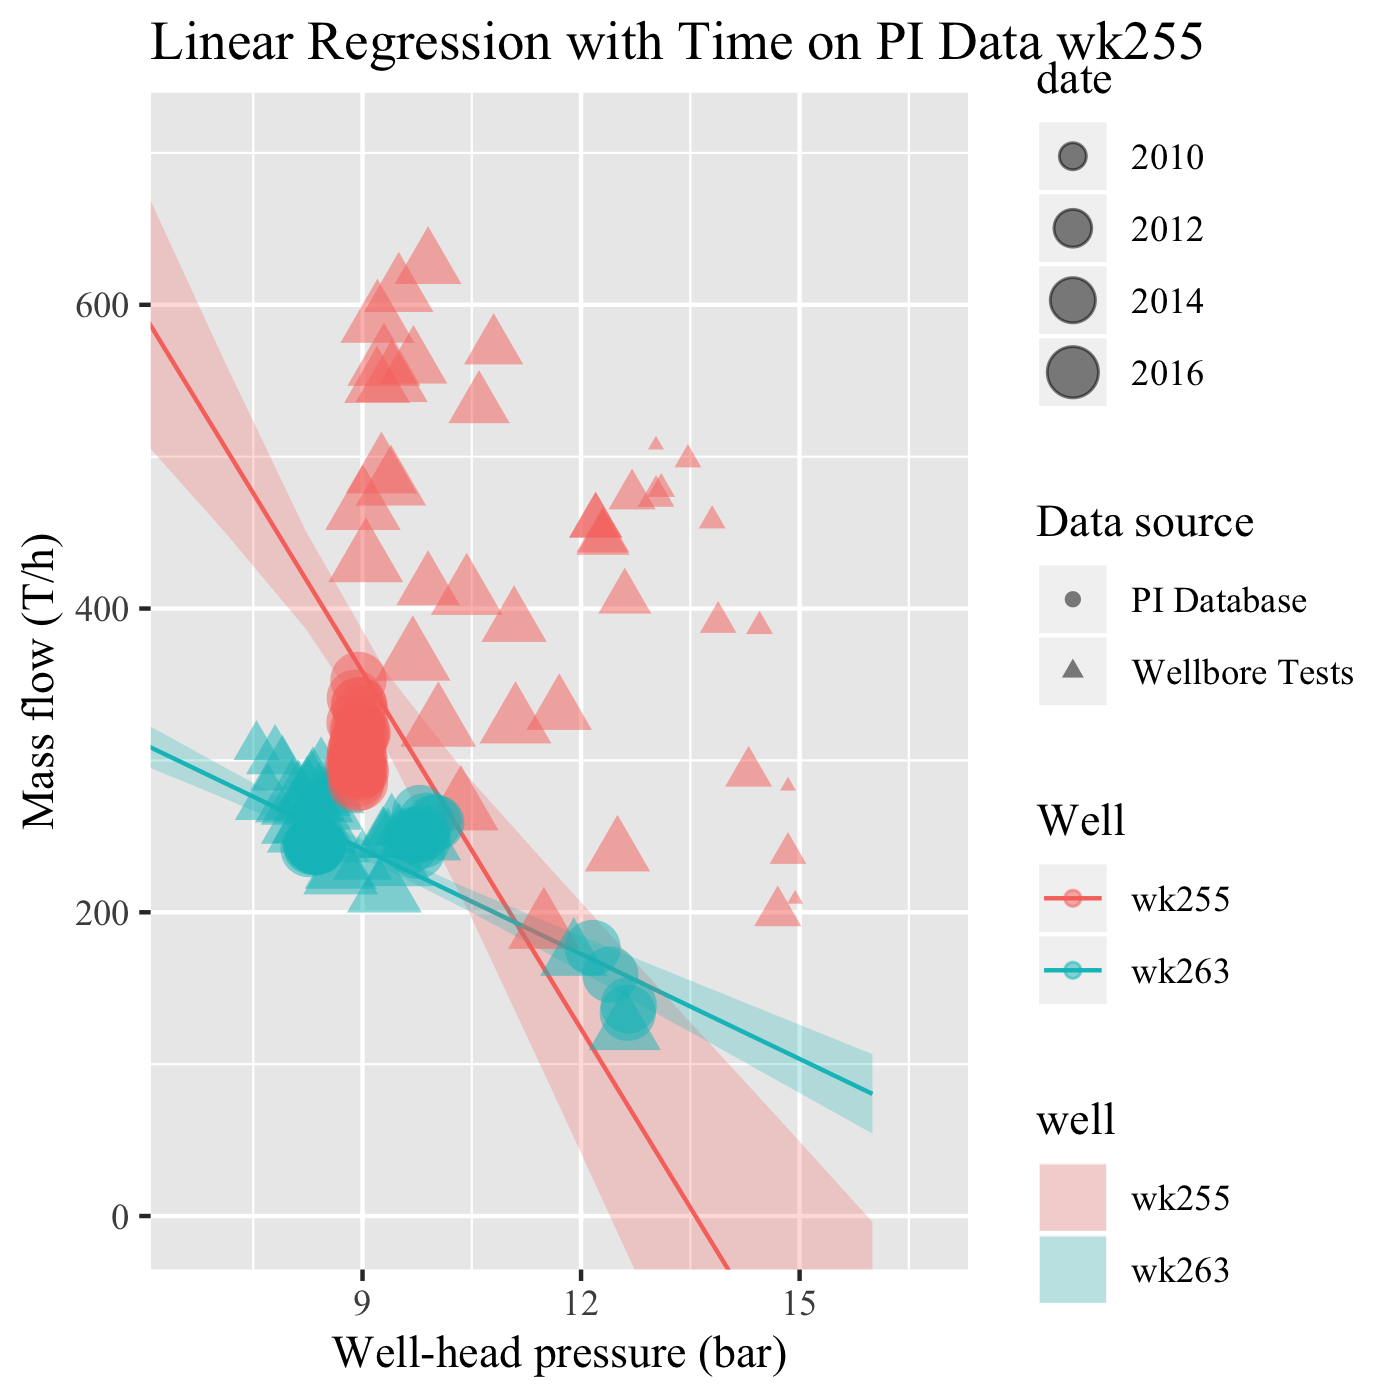
\includegraphics[width=\linewidth]{media/production_curve}
  \captionof{figure}{Two fitted production curves, forecasted one day in the future for December 1st, 2017. We expect it to fit closely to the most recent data because time is included as a regressor. The shaded region shows the 95\% credible intervals.}
  \label{fig:production_curve}
\end{minipage}
\end{figure}

Well-to-flash-plant assignment is specified in the configuration spreadsheet. Although most well/flash-plant relationships are fixed by the physical pipes, there is a subset of wells that can swing between three flash plants, which have steam flow limits. The decisions for which wells flow to which flash plants can be optimised with a mixed-integer linear program \cite{Fox:2018}, chosen manually, or chosen by any arbitrary method.

To calculate mass flows and flow enthalpies entering a facility (both flash plants and generators), we use equations \ref{eq:fp_mf} and \ref{eq:fp_h}. Every node must be fed by at least one node, so a dummy well is included in Figure \ref{fig:full_network}.

\subsubsection{Generator Flows and Power Conversions}
During pre-processing, three dummy nodes per generator for each type of flash plant output are placed in the network before the actual aggregated generator. In Figure \ref{fig:full_network}, there is a dummy for each type of fluid flow: intermediate pressure (IP), low pressure (LP), or water (W). Whether these are actually used depends on the configuration inputs. For instance, the binary \emph{BIN} plant will only ever use the \emph{BIN\_w} dummy because in reality, it is a waste to send steam to the low-efficiency binary generator.

Dummy generators flow into their respective generator. Contact Energy calculates power output as a function of the bulk mass flow by Equation \ref{eq:power}. These efficiencies are given to us in units of T/h/MW. Our uncertainty in the conversion factor is $\pm5\%$, which we interpret as $\eta \sim \text{Unif}\left( 0.95\overline\eta, 1.05\overline\eta \right)$, which holds for small ($<$10\%) percentages.

\subsection{Monitoring}

Monitors are how JAGS returns posterior samples to the user. There are three types of monitors:

\begin{enumerate}
\item Mean/variance, showing the current mean/variance of a parameter up to and including a sample. We are not interested in mean and variance because the same information can be extracted from the trace.
\item DIC (deviance information criterion), to evaluate goodness of fit of the model to the data. DIC is used to validate the model structure during development, but is not part of the final product. Also, graphical goodness-of-fit techniques are preferred because an informed user can identify specific issues such as residual errors.
\item Trace, showing every sample of a parameter. We use these to sample from the stationary distribution.
\end{enumerate}

The first monitor we set is on the well regression, predicting for a range of covariates to build a picture of the production curves. Examples of these curves are shown in Figure \ref{fig:production_curve}.

Next, we monitor mass flows at each facility and their probability densities. An example of its interpretation is given in Figure \ref{fig:bayesdemo}. These estimates for uncertainty are the strength of Bayesian inference; we can sample from the posteriors at the wells and propagate our uncertainty through the network to find the uncertainties at other locations.

\begin{figure}
\centering
  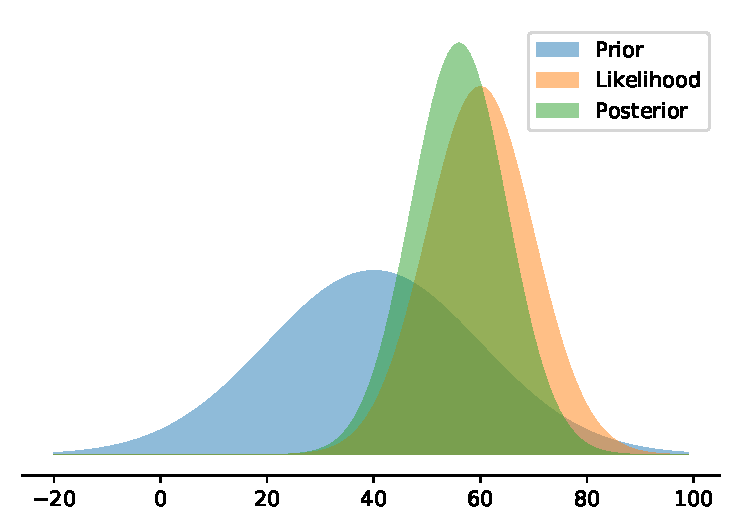
\includegraphics[width=0.5\linewidth]{media/bayesdemo}
  \captionof{figure}{The prior and likelihood functions multiply to give a posterior parameter distribution. The posterior is what we are interested in after observing the data. The uncertainty in the parameter is represented by the width of its distribution; conversely, the precision can be interpreted as the height of its peak because densities integrate to one. }
  \label{fig:bayesdemo}
\end{figure}

\subsection{Diagnostics}
One of the difficulties with MCMC approximations is they often require a burn-in (warm-up) period before settling into the stationary distribution of the Markov chain. Only the stationary distribution corresponds to the joint distribution we are interested in. In most practical uses, there is no way to predict convergence, so it must be done by monitoring the sample trace and running diagnostic tests.

\begin{figure}
\centering
  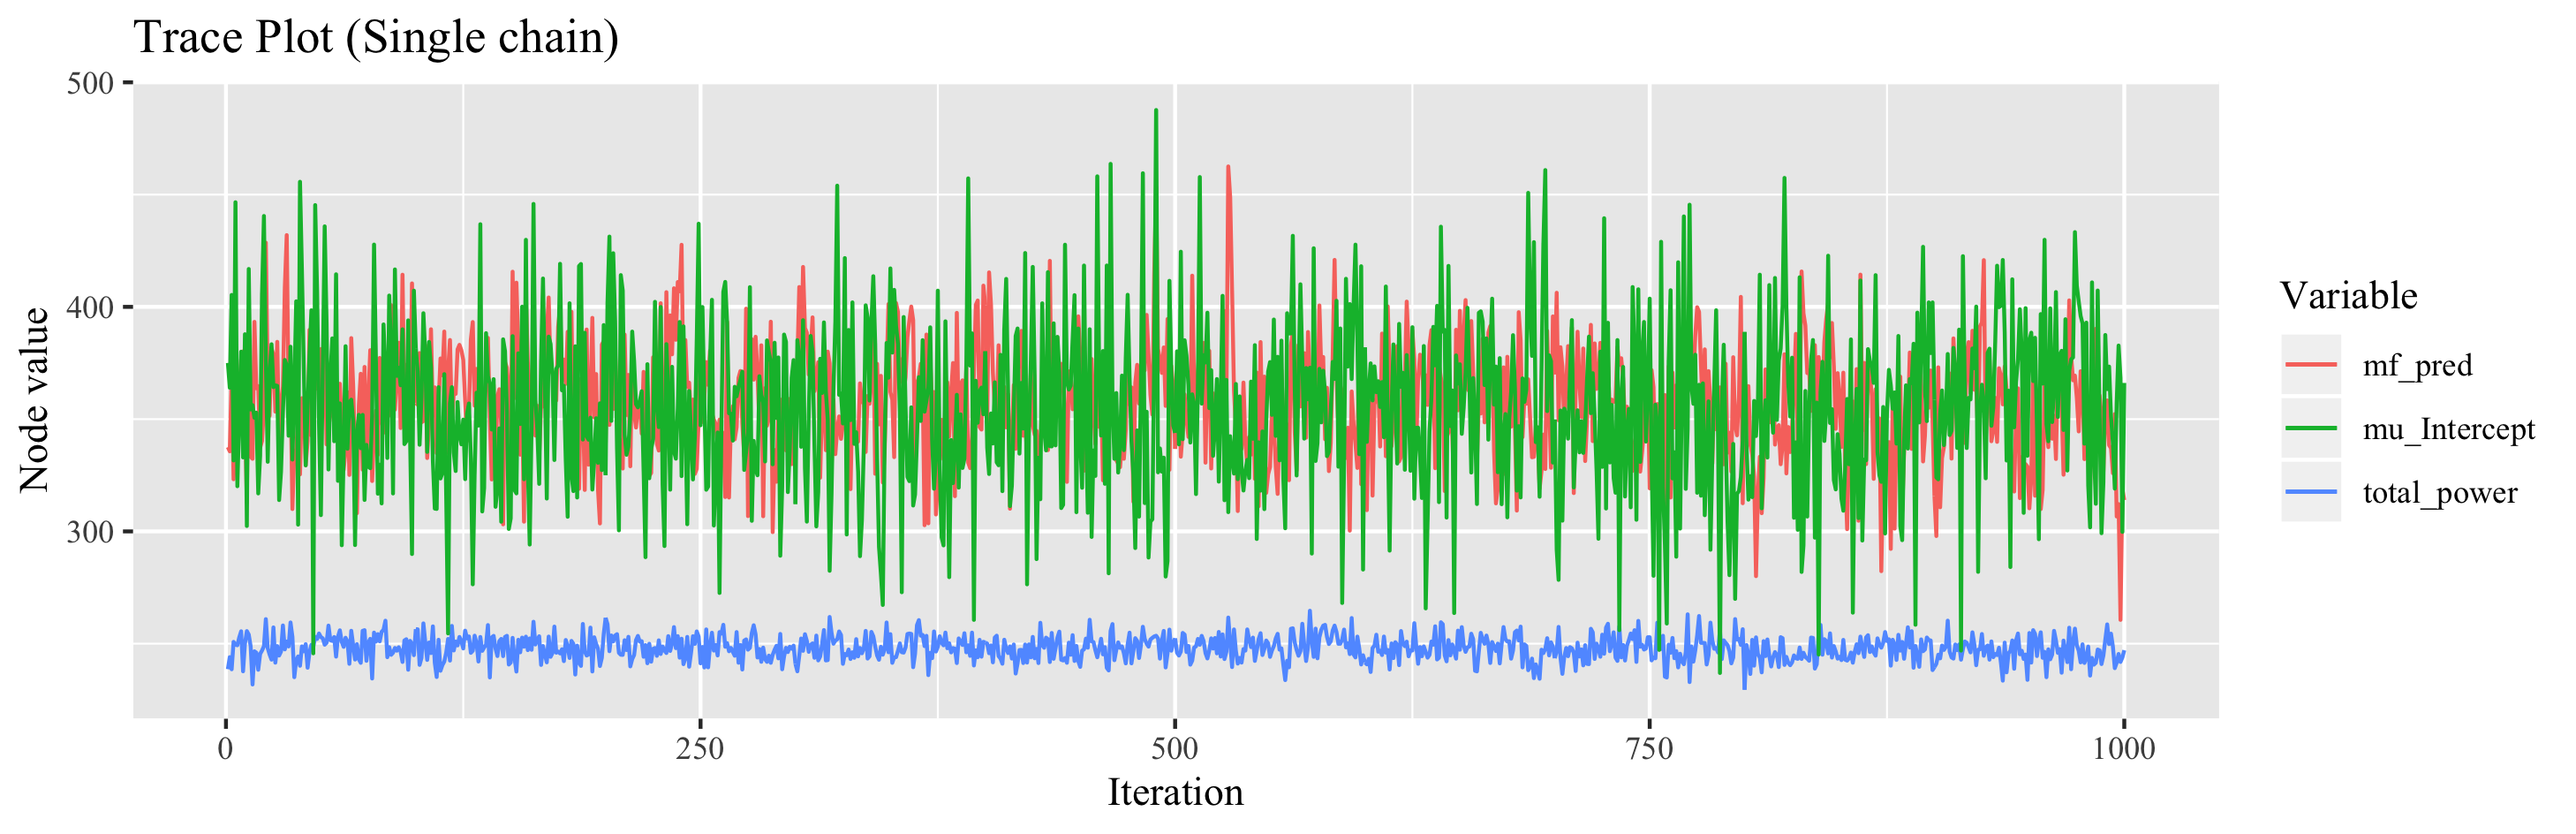
\includegraphics[width=\linewidth]{media/trace_plot}
  \captionof{figure}{Example trace plots displaying normal behaviour. The sampler appears to have reached its equilibrium distribution with no trend.}
  \label{fig:trace_plot}
\end{figure}

Poor convergence or mixing is represented by a strong trend at the beginning of the trace plot. This is not present in Figure \ref{fig:trace_plot}, but visual analysis of trace plots for every parameter.
JAGS provides other diagnostic tests in the CODA package. There are two main tests to confirm this:

\subsubsection{Geweke's Convergence}
Geweke's convergence diagnostic for MCMC samples tests for equality of the means in the first 10\% and last 50\% of the trace (the samples in iteration order). The means will be equal if the sample is drawn from a stationary distribution, indicating the burn-in period has been successfully excluded. Geweke's statistic has a T-distribution using the following T-test statistic:
\begin{equation}
z=\frac{\overline{X_1}-\overline{X_2}}{\sqrt{\frac{s_1^2}{n} + \frac{s_2^2}{m}}}
\end{equation}
where $\overline{X_1}$ and $\overline{X_2}$ are the sample means of the first 10\% and last 50\% of the samples, $s^2$ are their corresponding standard variances, and $n$ and $m$ are the number of samples in the two groups. The results of Geweke's test for 100 randomly selected parameters are shown in Figure \ref{fig:geweke}.

\begin{figure}
  \centering
  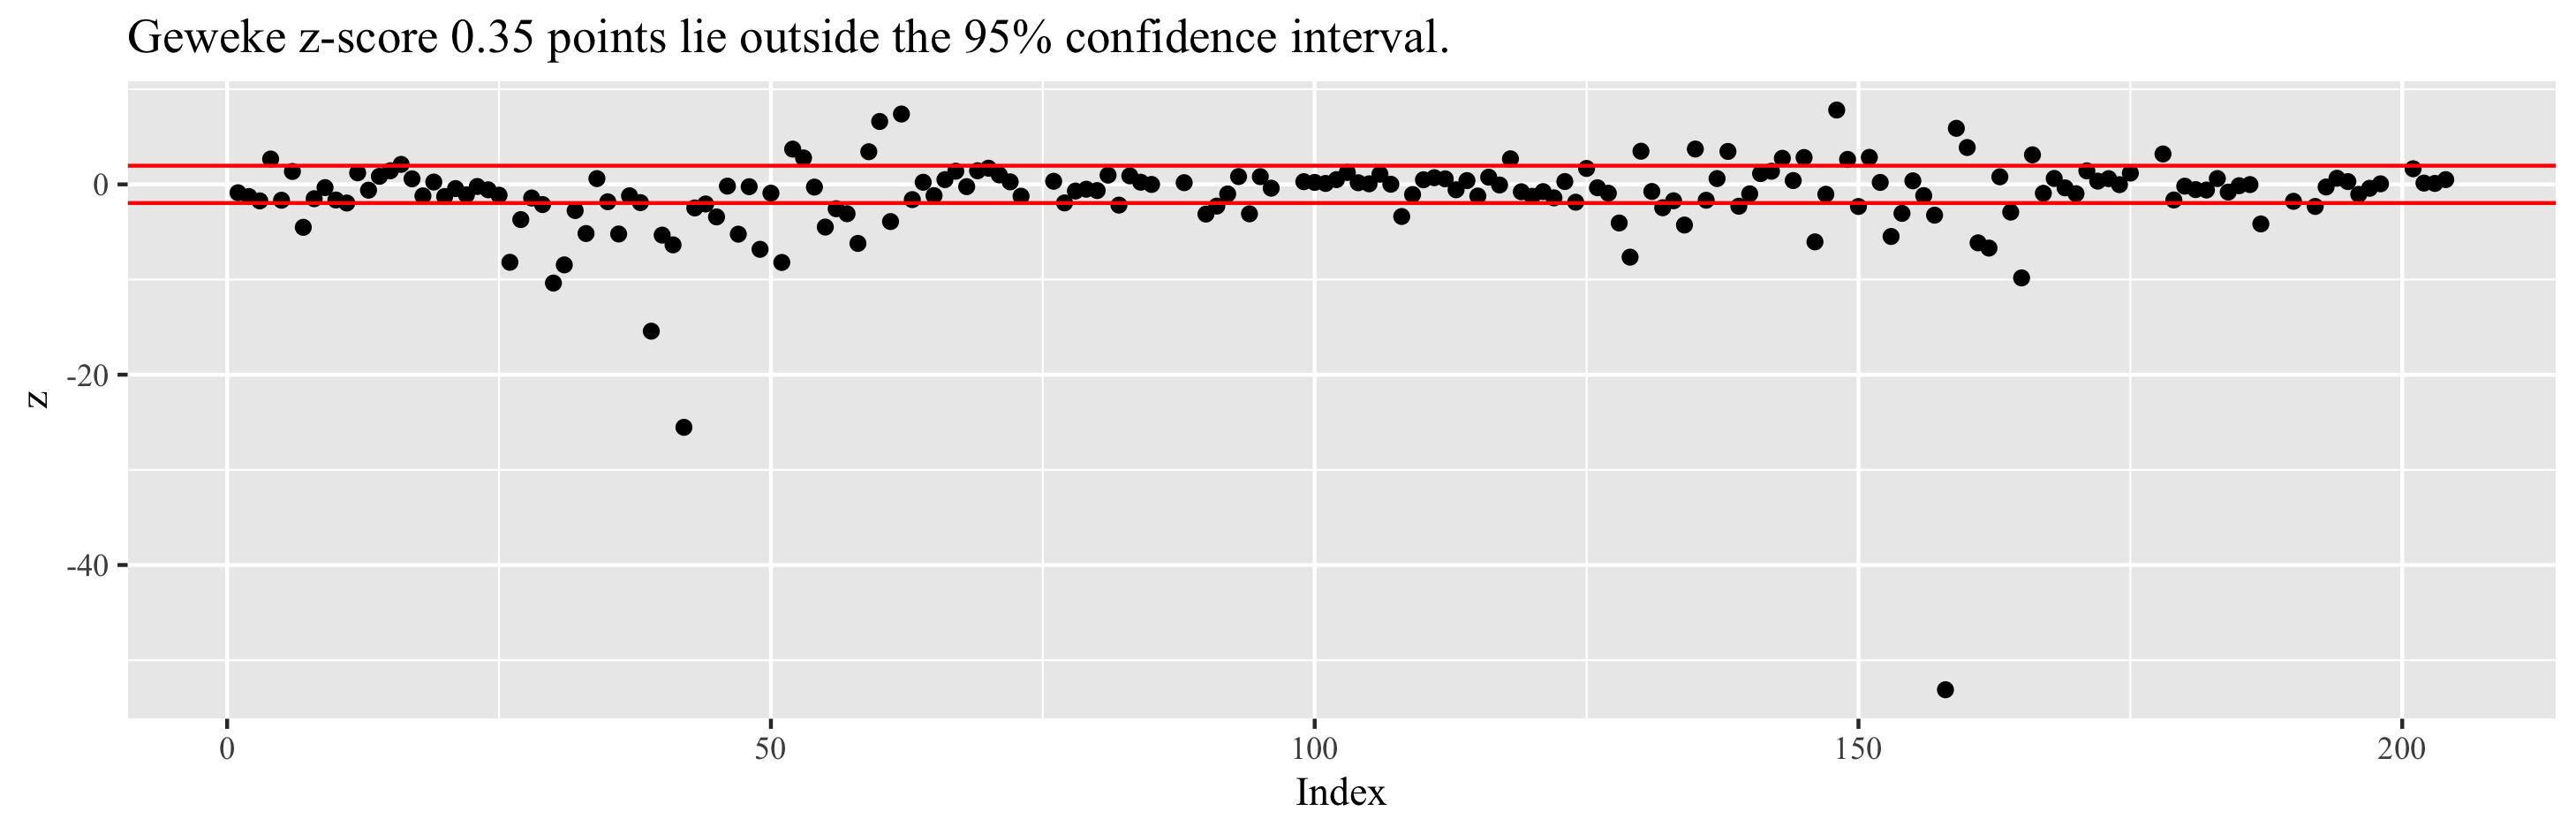
\includegraphics[width=\linewidth]{media/geweke}
  \captionof{figure}{More than 5\% of z-scores outside the confidence interval, indicating the chains have not converged and are not long enough, or they contain burn-in.}
  \label{fig:geweke}
\end{figure}

If true univariate convergence has been achieved (multivariate convergence is much more difficult to test for), we expect 95\% of variables to pass Geweke's test with a z-score (a Normal approximation of the T-statistic) less than 1.96 with 95\% confidence. However, the changes in the power output traces were significant, so a short burn-in of 200 iterations was introduced and the number of iterations was increased to 10,000. This is conservative -- satisfactory plots were obtained with 1,000 iterations or about one minute of run-time.

\subsubsection{Gelman-Rubin Potential Scale Reduction Factor}
The Gelman-Rubin convergence diagnostic gives the potential scale reduction factor (PSRF) for each parameter. This requires at least two independent, parallel chains beginning from over-dispersed (different) starting positions, and tests whether the chains have converged to identical distributions. If the chains have not converged, the scale reduction factors will have upper confidence limits greater than one. It is therefore possible that when run indefinitely, the variance of the parameter estimate could shrink by the PSRF \cite{Gelman:1992}.

Executing Gelman's test on all monitored parameters runs into issues with an internal Cholesky matrix factorisation of an ill-conditioned matrix. Testing a smaller selection yields Table \ref{tab:gelman}.

% latex table generated in R 3.4.2 by xtable 1.8-2 package
% Fri Sep 14 00:11:12 2018
\begin{table}[h]
\centering
\begin{tabular}{rr}
  \hline
Point est. & Upper C.I. \\ 
  \hline
1.00 & 1.00 \\ 
  1.00 & 1.01 \\ 
  1.00 & 1.01 \\ 
  1.00 & 1.03 \\ 
  1.00 & 1.02 \\ 
  1.00 & 1.00 \\ 
  1.00 & 1.02 \\ 
   \hline
\end{tabular}
\caption{Select potential scale reduction factors from Gelman's diagnostic test.} 
\label{tab:gelman}
\end{table}


Some of the upper CIs are slightly greater than one, but not significantly. We can expect their credible intervals and standard errors are approximately the correct width. Running the simulation for longer will shrink the CI, but for how long is a balance between computational resources and the need for precision -- large PSRFs are acceptable if they are in components of the network that do not affect parameters of interest.

%%%%%%%%%%%%%%%%%%%%%%%%%%%%%%%%%
\section{Results}
Contact Energy has provided wellbore test data up to early 2018 and PI logs up to the end of December 31. They also supplied an example calculation for December 1st, 2017. To test the forecasting ability of our model, we discard all data after November 30th, 2017, and compare predicted mass flows with measured flows for December 1st. The traces are analysed in R, and the names of potentially sensitive facilities have been obfuscated. Because there are so many facilities and parameters to monitor, the plots in this section may only include a subset of facilities that represent the different outcomes present in the simulation.

A word of caution: we treat CEL's calculations as the ground truth in Section \ref{sec:downflow}. In reality, the figures provided by CEL will include an unknown bias induced by any method of calculation, and an unknown variance due to measurement and other errors. The comparison outcomes should therefore be treated qualitatively to assess whether our model is working, rather than to assess numerical accuracy.

\subsection{Well Production Curves}

We compare production curves before and after including PI data in Figure \ref{fig:production_curve_comparison}. PI data has changed the regression for w145 slightly, but in the proximity of the data (where we might want to make predictions), the regression is almost exactly the same.

The regression for w93A has adjusted to fit the PI data more closely in the well-head pressures of the PI data. Therefore, we know that the PI data does not agree perfectly with the well test data -- however, we trust the PI data for our predictions because it is the most recent. A consequence of this disagreement is the parameters estimate depends on how much PI data we add -- Figure \ref{fig:production_curve_comparison}, right, shows 60 days and drastically affects the regression despite being only two months of eight years of data. Since PI data is taken from $n$ consecutive days, it is similar to weighting one point by $n$ and giving it disproportionate influence over the regression compared to the other points. We conclude that although PI data is up-to-date, adding it can decrease the accuracy of the production curve parameters.

\begin{figure}
  \begin{subfigure}[b]{0.5\textwidth}
    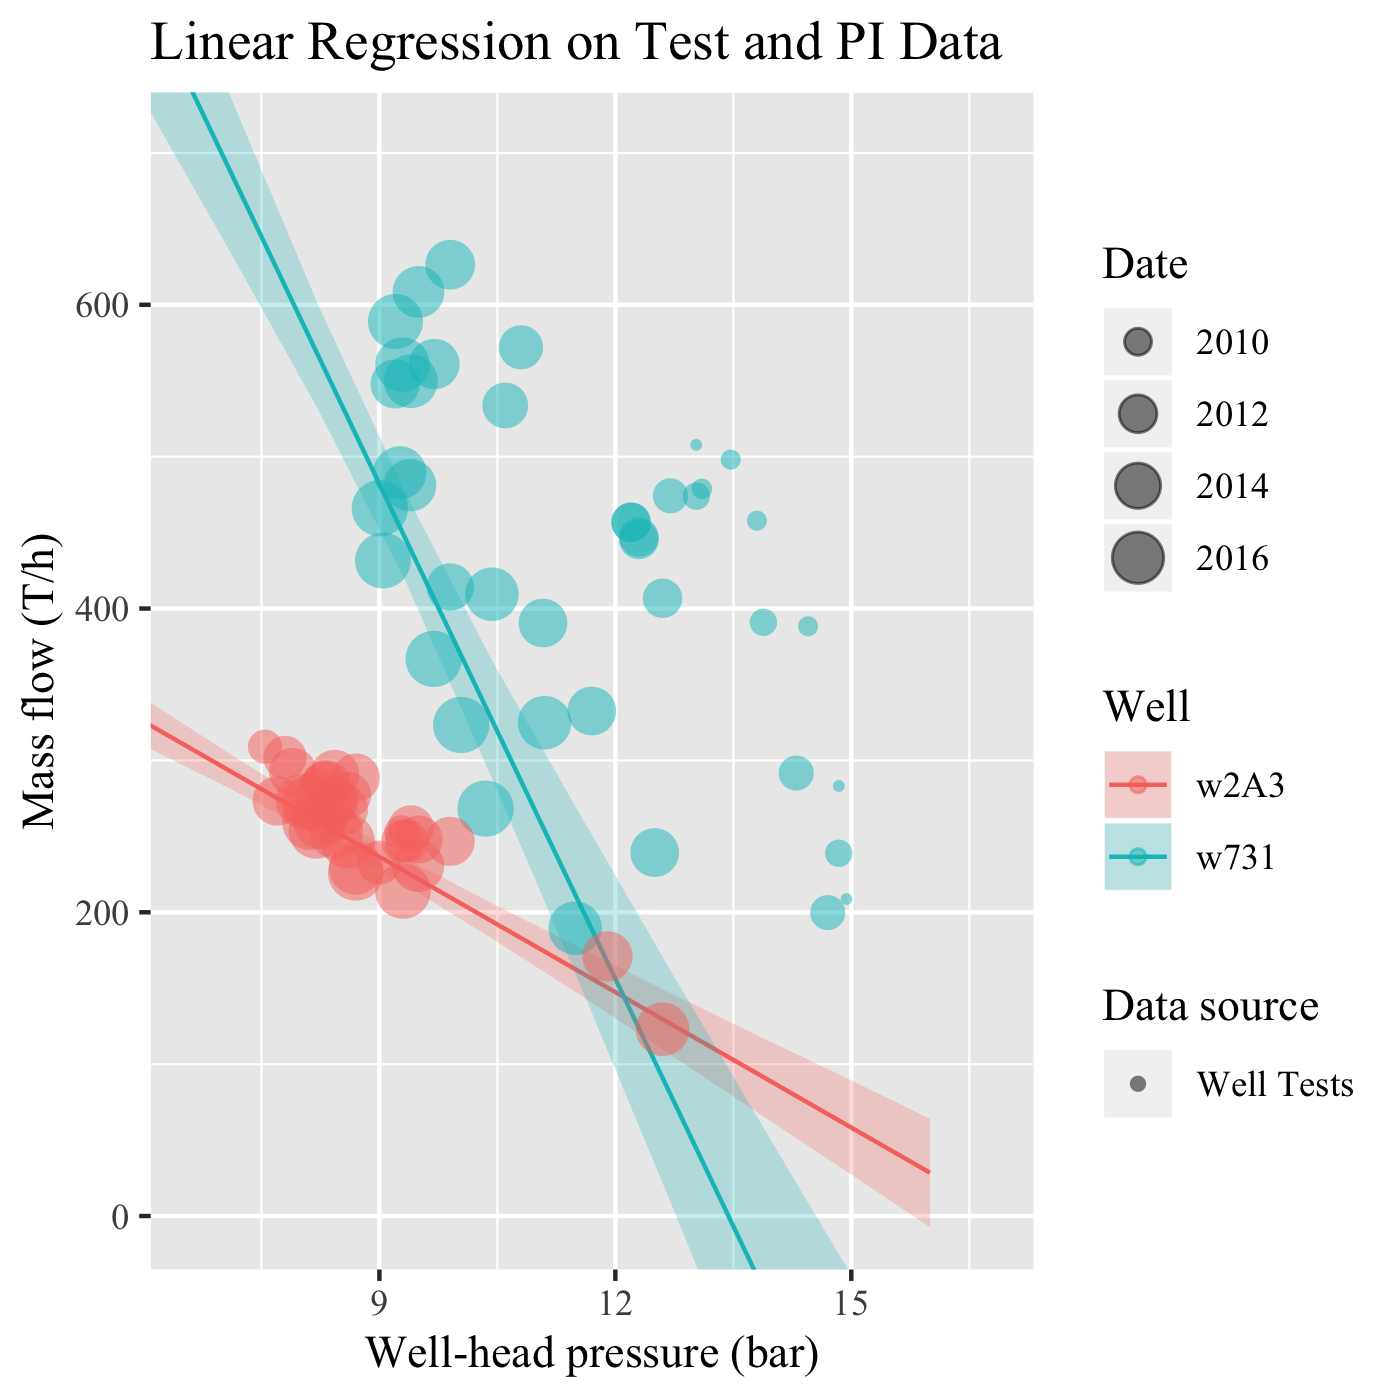
\includegraphics[width=\textwidth]{media/production_curve_without}
  \end{subfigure}
  \hfill
  \begin{subfigure}[b]{0.5\textwidth}
    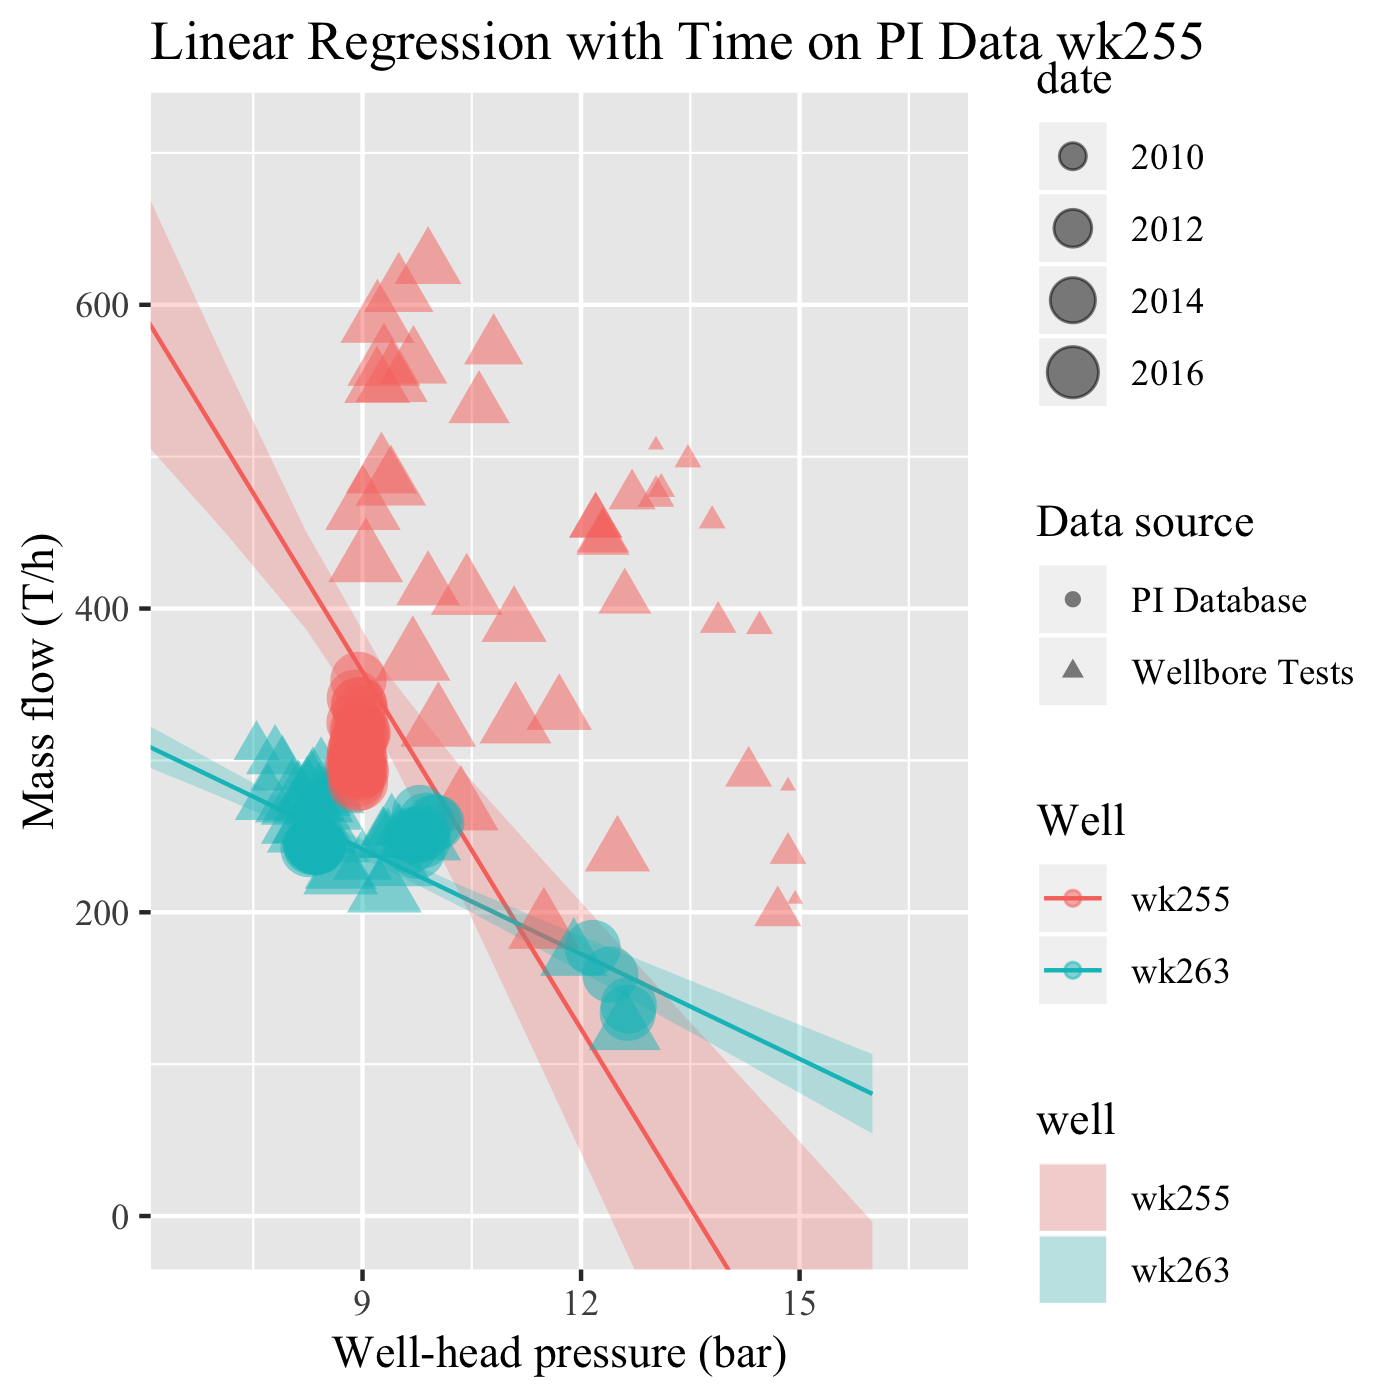
\includegraphics[width=\textwidth]{media/production_curve}
  \end{subfigure}
  \caption{Left: Just well test data. Right: After including PI data. We expect the curves to make better predictions near the PI data after inclusion. Forecasted production curves for December 1st, and shaded regions are 95\% credible intervals.}
  \label{fig:production_curve_comparison}
\end{figure}

\subsection{Well Mass Flows}
\begin{figure}
\centering
  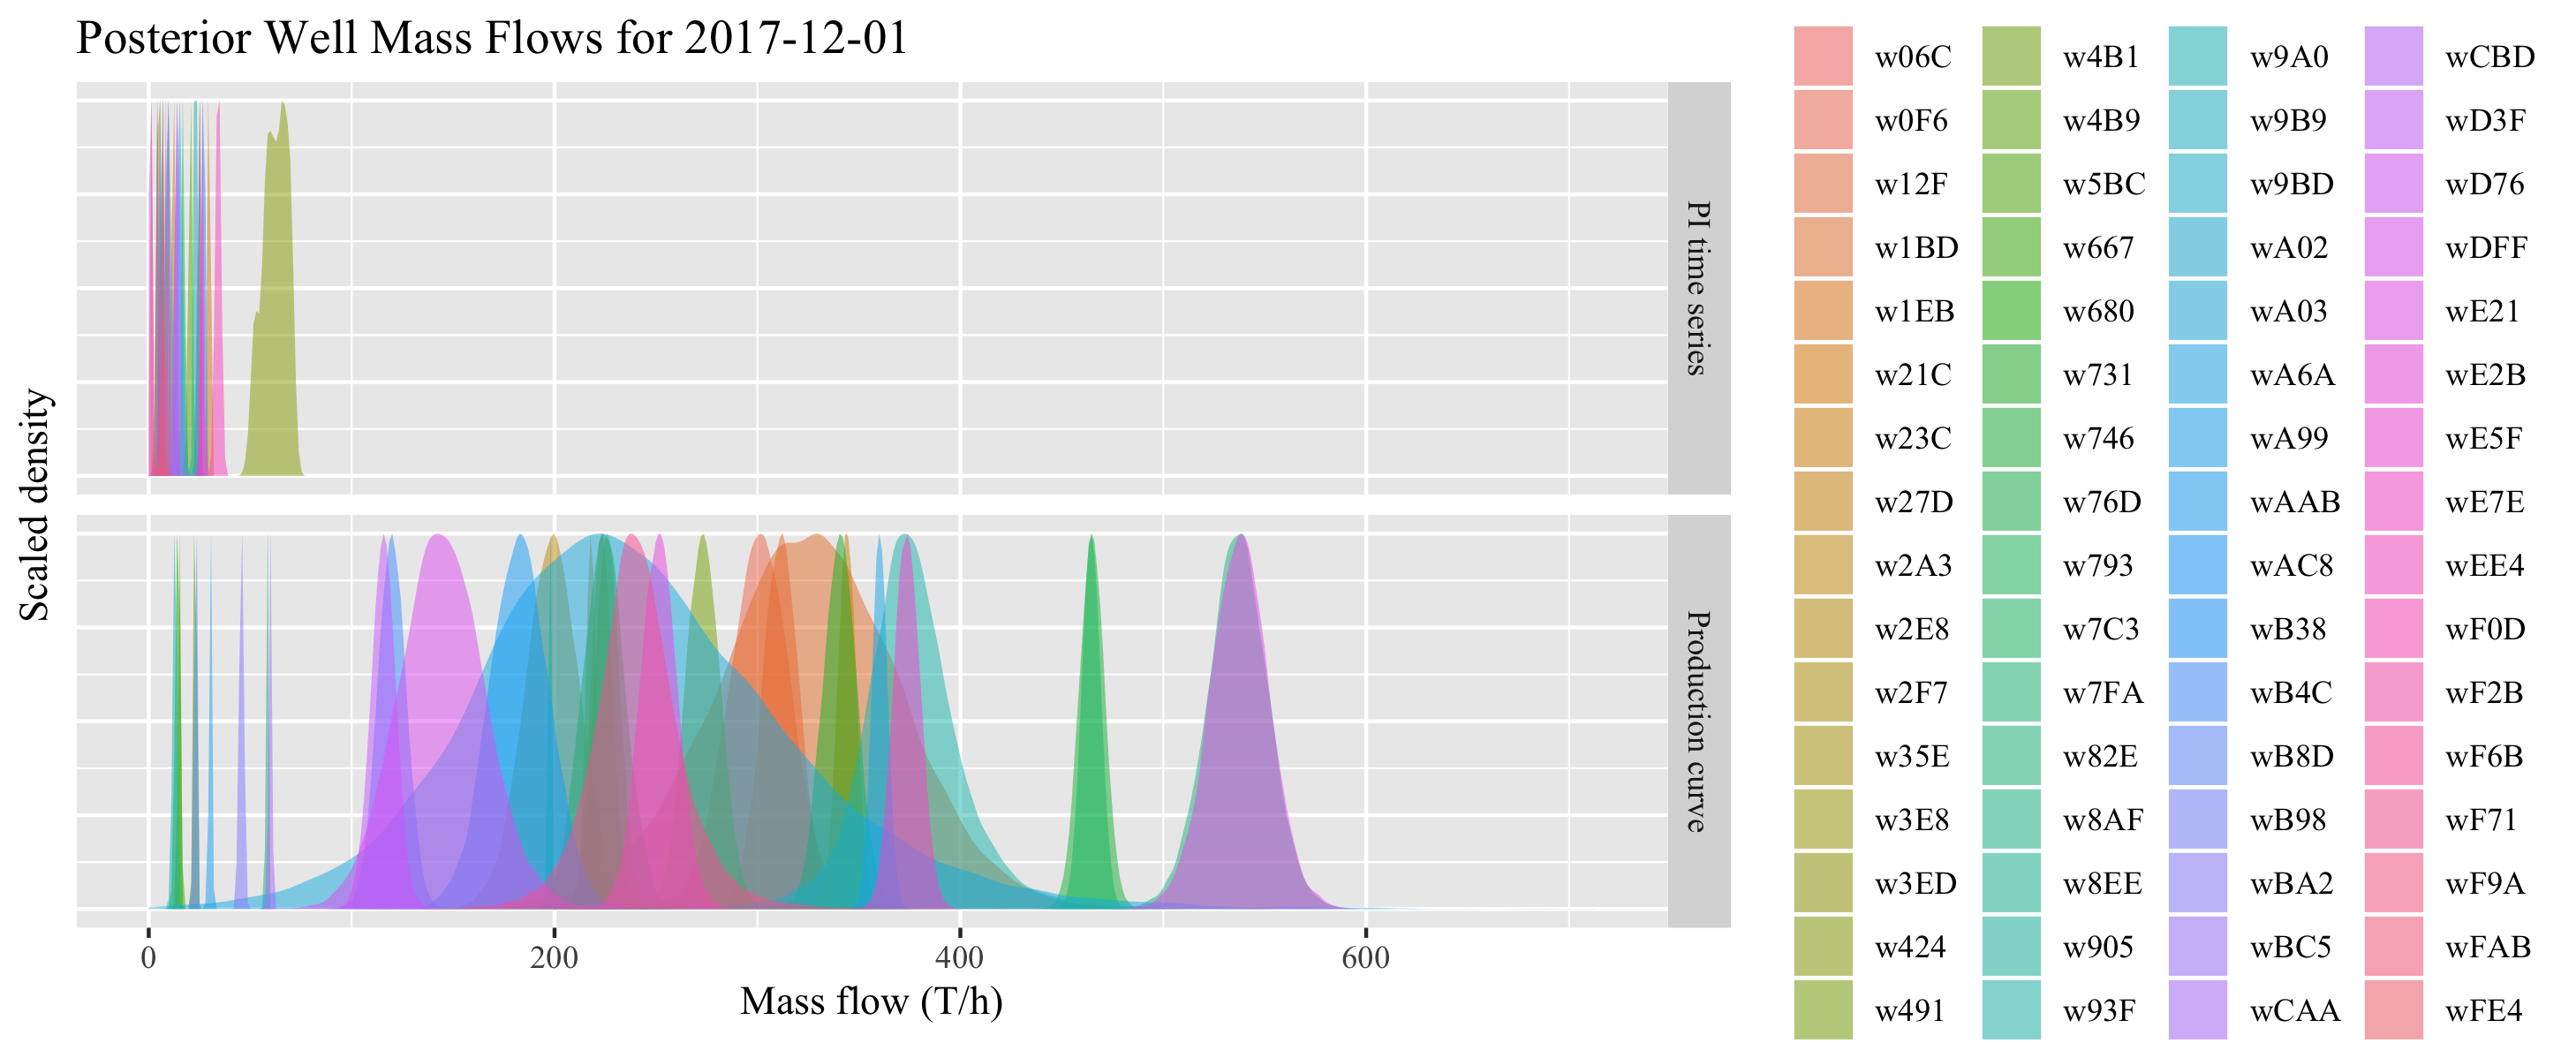
\includegraphics[width=\linewidth]{media/mf_wells}
  \captionof{figure}{Posterior mass flows for all 71 wells, divided into wells with production curves and wells with a simple time-series (see Figure \ref{fig:ts_experiment} for time-series examples). Wells show large variations in mean mass flow and variance.}
  \label{fig:mf_wells}
\end{figure}

Figure \ref{fig:mf_wells} presents the posterior densities for mass flow at selected wells. We can see that some wells have more variation than others. Variance can either come from the regression model or the data, with issues including:

\begin{enumerate}
\item Lack of data to fit the regression.
\item Data is for pressures and times far away from the values used for prediction; e.g. very old data that is no longer relevant.
\item Mass flow is non-linear with pressure and time (i.e. bad fit).
\end{enumerate}

We do not see any issues with non-linearity in the diagnostic plots (Figure \ref{fig:diagnostics}), and know from previous DIC comparisons that higher order terms do not significantly aid the regression. Therefore, we will next look at the data. We can compare the performance of well predictions by comparing well standard deviations by their data sources.

\begin{figure}
  \centering
  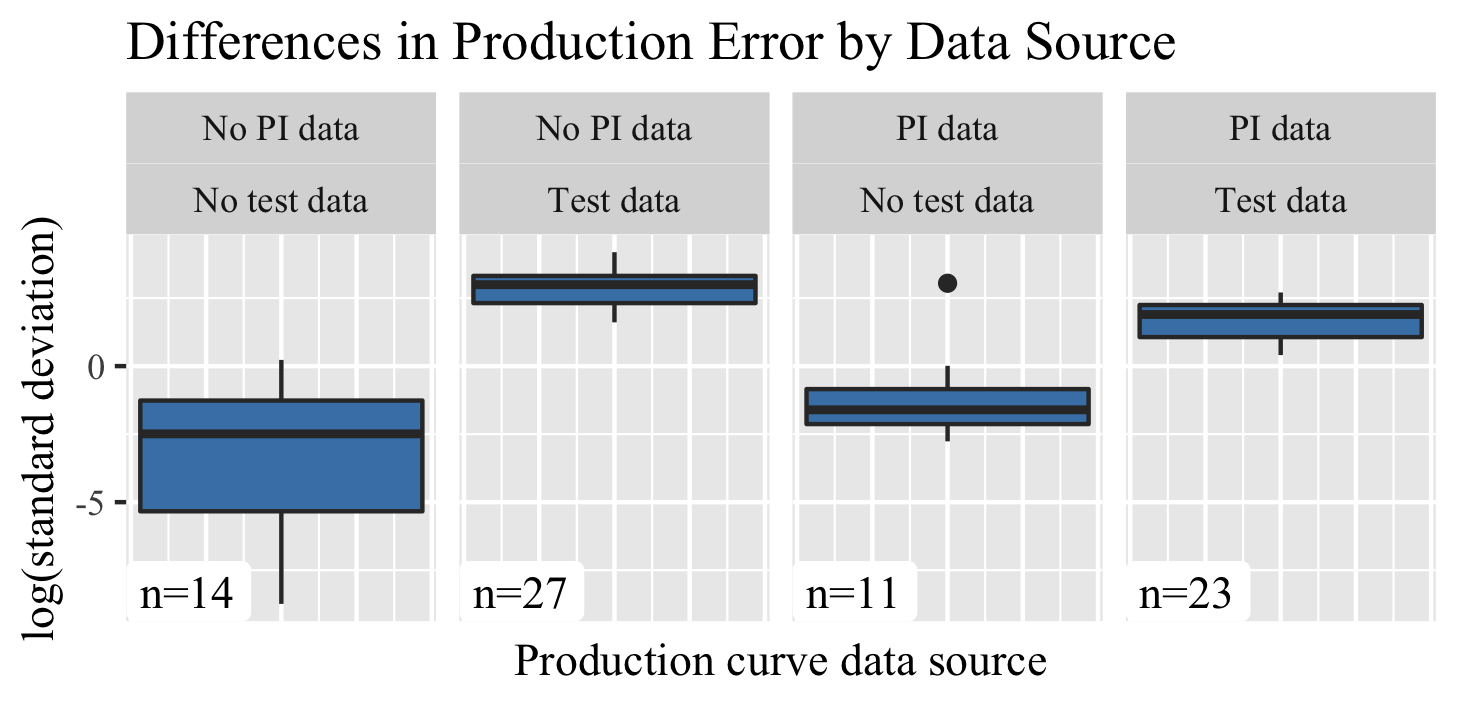
\includegraphics[width=.5\linewidth]{media/error_source}
  \captionof{figure}{Facets of the data sources for the production curve. No data (far left) means there was no curve -- these mass flows were predicted by time series on PI mass-flow data. $n$ is the number of wells, and standard deviation is calculated as $\text{sd}(\hat{\dot{m}}_j)$ for each well.}
  \label{fig:error_source}
\end{figure}

Figure \ref{fig:error_source} shows that the most precise wells are predicted by time series, rather than production curve. This is not surprising -- by predicting from a production curve of mass flow by well-head pressure and time, we introduce intermediate errors. The other three facets with production curves suggest that test data is the source of variance in the regression. We class the data sources in Table \ref{tab:data_sources}.

\begin{table}
\centering
\begin{tabularx}{0.85\linewidth}{rXX}
\hline
 & Well tests & PI data \\ 
  \hline
Variance & High & Low  \\
Period & Long-term, 2002-2017 & Very recent, since the last change in configuration \\
Effective for & Short-term time-series prediction & Production curve and parameter estimation \\
   \hline
\end{tabularx}
\caption{Differences in the two data sources}
\label{tab:data_sources}
\end{table}

\subsection{Individual Well Declines}

% latex table generated in R 3.4.2 by xtable 1.8-2 package
% Thu Sep 20 12:22:42 2018
\begin{table}[h]
\centering
\begin{tabular}{lrrrr}
  \hline
well & Mean & Lower 2.5\% & Upper 97.5\% & n \\ 
  \hline
w06A & -0.021 & -0.039 & -0.000 &   10 \\ 
  wA2E & -0.272 & -0.332 & -0.214 &   88 \\ 
  wF8E & 0.010 & -0.035 & 0.048 &    4 \\ 
   \hline
\end{tabular}
\caption{Credible intervals for $\beta_\text{date}$ in units T/h/d. $n$ is the number of test data points rather than the total including PI data, because PI data is from a single month and cannot estimate the $\beta_\text{date}$ parameter on its own. Full table in Table \ref{tab:beta_date_all}.} 
\label{tab:beta_date}
\end{table}


Table \ref{tab:beta_date} presents credible intervals for decline at selected wells. The rates are mostly negative (in decline), but some rates are not statistically significant, such as wF8E where a rate of zero is within the credible interval.

There is varying precision in the decline -- wA2E is an example of a well with good precision in the decline rate. This is because there have been 88 recorded values with a range of covariate values, giving the parameter estimates good support, and most of the 88 observations agree with a declining rate.

High variance in regression parameters can either be due to a weak statistical correlation (high noise), or insufficient data to reject a null hypothesis. Inspection of well wF8E shows that there is insufficient well test data available. Four points is not enough to reliably estimate variance in a model with three parameters, even if the trend is strong. When precision is low, we cannot make strong claims about the decline rate for that well. However, we can say that at a fixed well-head pressure, mass output for well wA2E is declining between -0.214 and -0.332 T/h/d.

%\begin{figure}
%  \centering
%  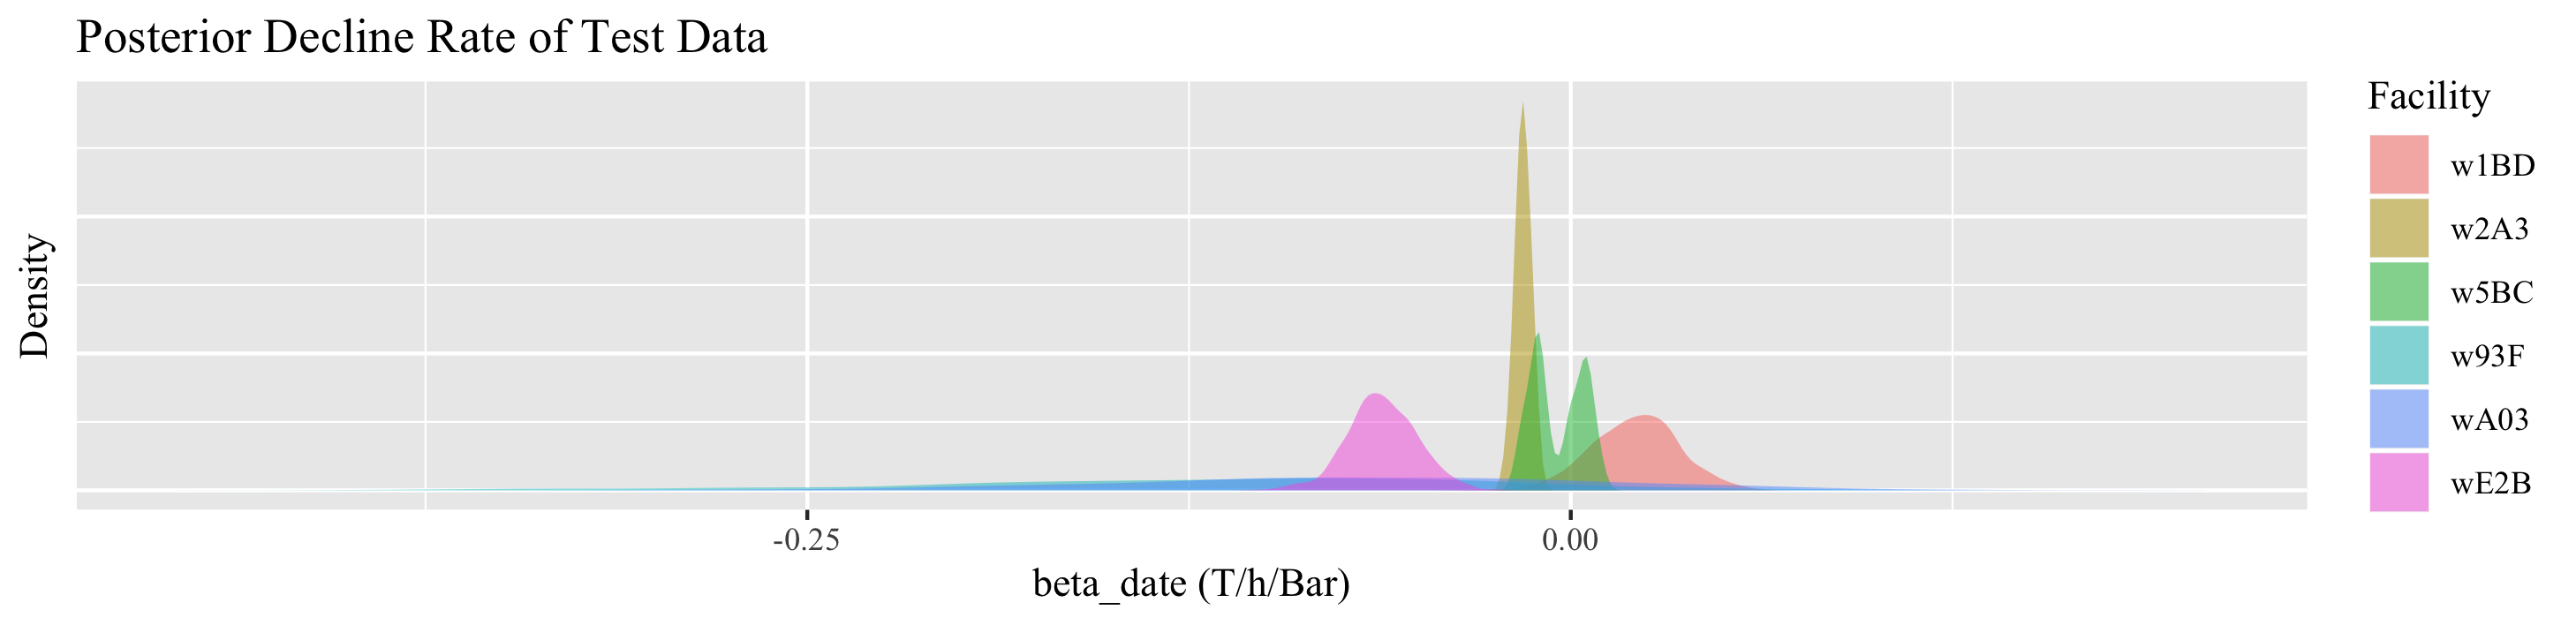
\includegraphics[width=\linewidth]{media/beta_date}
%  \captionof{figure}{Posterior decline rate of selected liquid wells.}
%  \label{fig:beta_date}
%\end{figure}

\subsection{Down-flow Results} \label{sec:downflow}
The results from the previous section propagate through the network to the flash plants and generators. We are most interested in the flash plants, where we have an example spreadsheet of flows for a particular day and constraints on steam flows.

\subsubsection{Flash Plant Mass Flow Verification}

After making predictions for the wells, we obtain mass flows entering the flash plants. This is split up into intermediate pressure, low pressure and water flows. We verify our posterior beliefs for these flows against an example calculation from CEL in Figure \ref{fig:verification}. 

% Good FPs: fp1, fp14, fp2, fp4, fp9-10
%       fp0D        fp66        fpEE        fpBC        fp6C        fp24        fp62        fp28        fpAD 
%      "fp5" "direct ip"       "fp1"       "fp4"    "fp9-10"      "fp14"      "fp15"      "fp16"       "fp2" 
%       fp76        fp8F 
%  "poi dry" "abandoned"
\begin{figure}
  \centering
  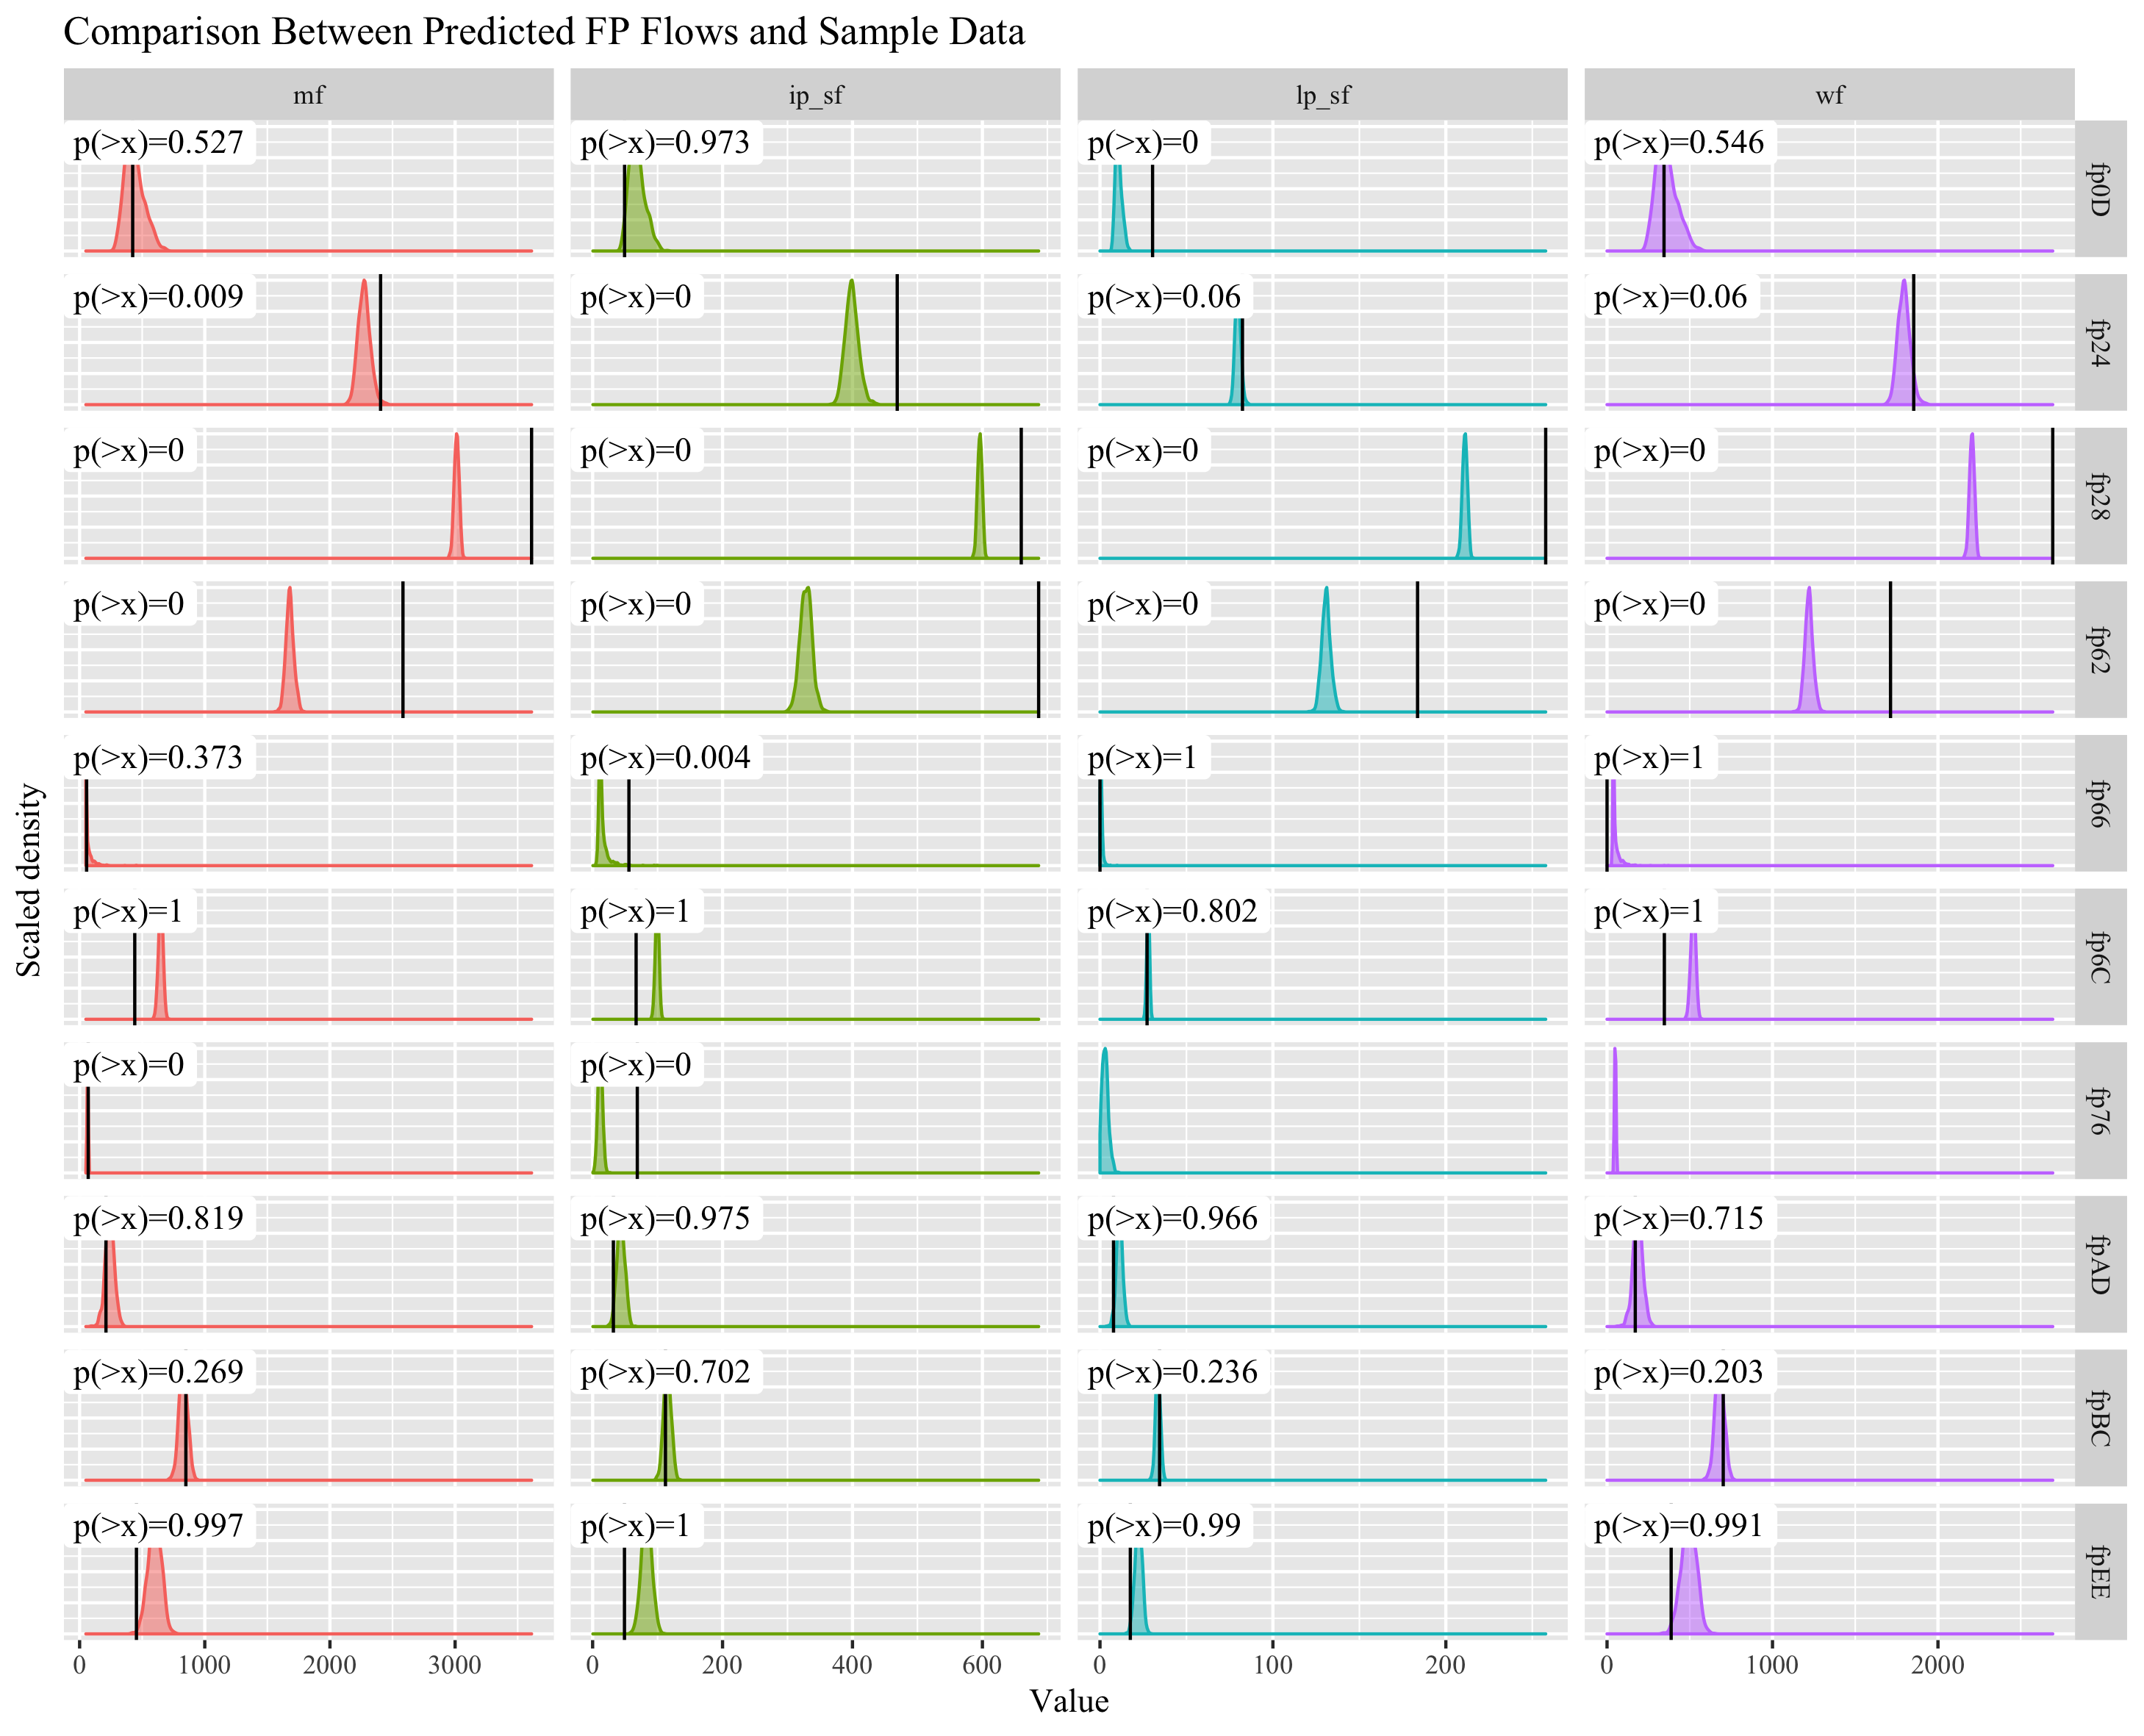
\includegraphics[width=\linewidth]{media/verification}
  \captionof{figure}{Verification of predicted flows with supplied calculations shows some disagreement ($p<0.025$ or $p>0.975$), if we assume CEL's figures as the ground truth. Densities are the model's forecasts and black lines are the given figures from CEL (estimated by CEL, not direct from the PI loggers).}
  \label{fig:verification}
\end{figure}

There are three main observations:

\begin{enumerate}
\item Even if not within 95\%, most of our estimates are similar.
\item fp24, fp62 and fp28 are all fed by wells that can be configured. However, fp62 seems to under-estimate total $\dot{m}$ and therefore all the other components of flow.
\item Some flash plants with high precision are very far from the CEL estimates, which makes it likely that our regression contains error for at least one of the wells.
\end{enumerate}

To investigate the difference between fp62 and fp24/fp28, we look at the data methods shown in Appendix \ref{sec:fpdata}. Many of the wells feeding fp62 have no test data, whereas most wells in fp24 and fp28 have substantial amounts of test data ($n_\text{test} > 20$). This suggests that test data has an important role in calibrating production curves for forecasts. However, this is not strong evidence and would need to be investigated further.

\subsubsection{Flash Plant Constraints}
Contact Energy defines constraints on the flows in the network. We can estimate the probabilities of each constraint being violated by the proportion of the trace exceeding the constraint value. However, more nuanced comparisons can be made with the density plot in Figure \ref{fig:constraints}.

\begin{figure}
\centering
  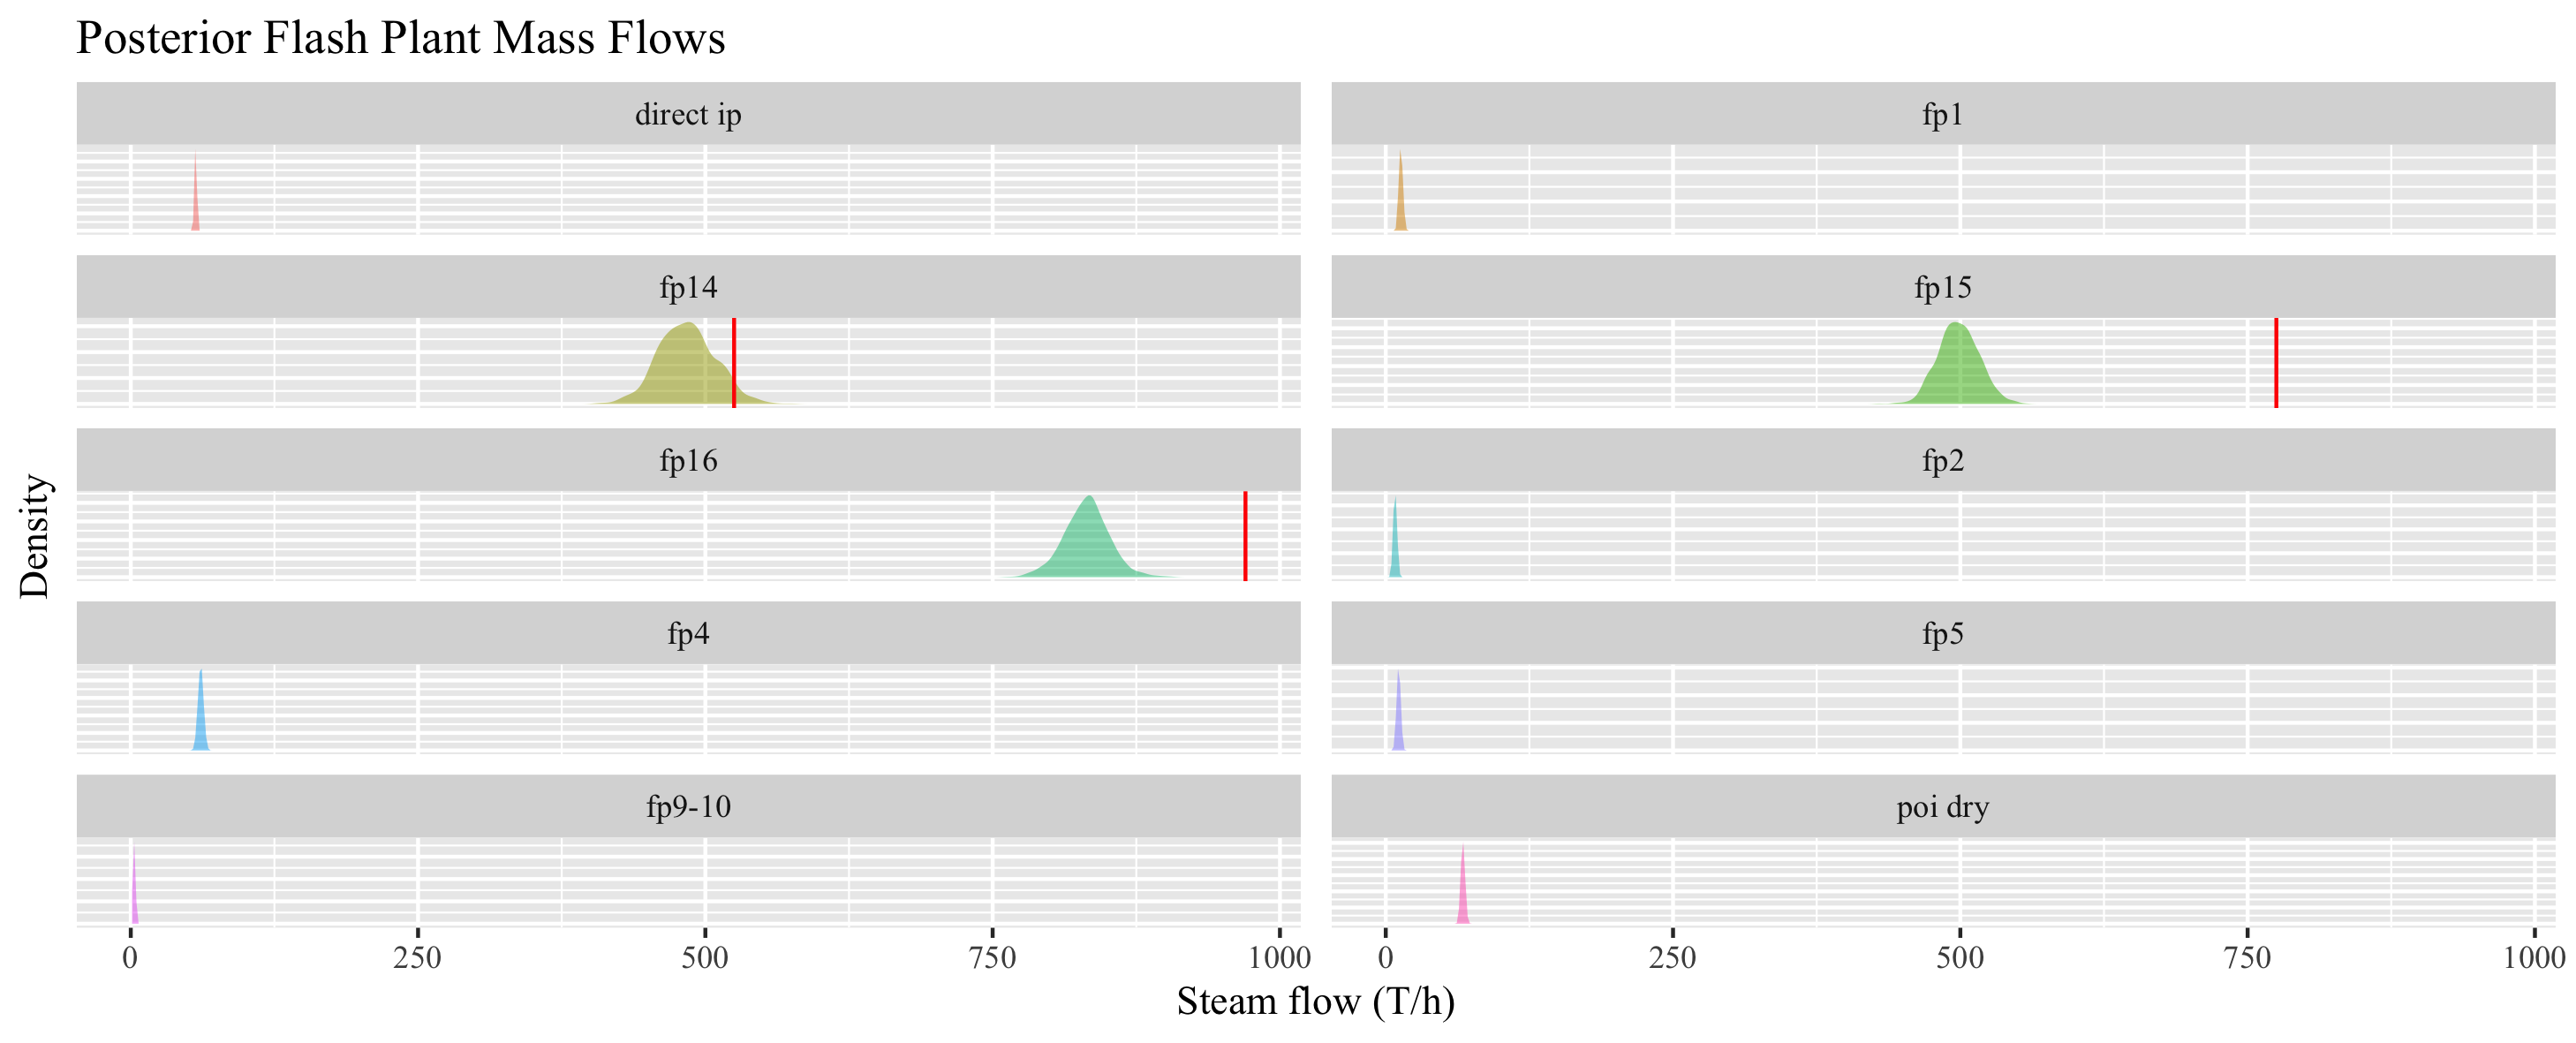
\includegraphics[width=\linewidth]{media/constraints}
  \captionof{figure}{Posterior density plot of the steam flows through the flash plants. Known steam limits are shown by a vertical red line. The expected probability of a constraint violation is the proportion of the density above the limit.}
  \label{fig:constraints}
\end{figure}

Some of the flows are under-estimated because data is not available for all wells. In Figure \ref{fig:constraints}, we can see that all of the flash plants are operating below their limits in the December 1st configuration. However, one flash plant (fp24, one of the flash plants where wells can be redirected) is more likely to violate its constraints than the others, suggesting that one or more wells should be redirected to another flash plant.

\subsubsection{Generator Flows and Power}
The mass flows into the generators and their respective power outputs are shown in Figure \ref{fig:gens}. We show that our model can propagate uncertainty through to the generators' power estimates, and that they are relatively disperse. We found that our Poihipi and Te Mihi power generation estimates have large discrepancies compared with the actual PI readings, but this issue is difficult to diagnose because it is likely to stem from how we convert steam to power, or our network structure.

\begin{figure}
\centering
  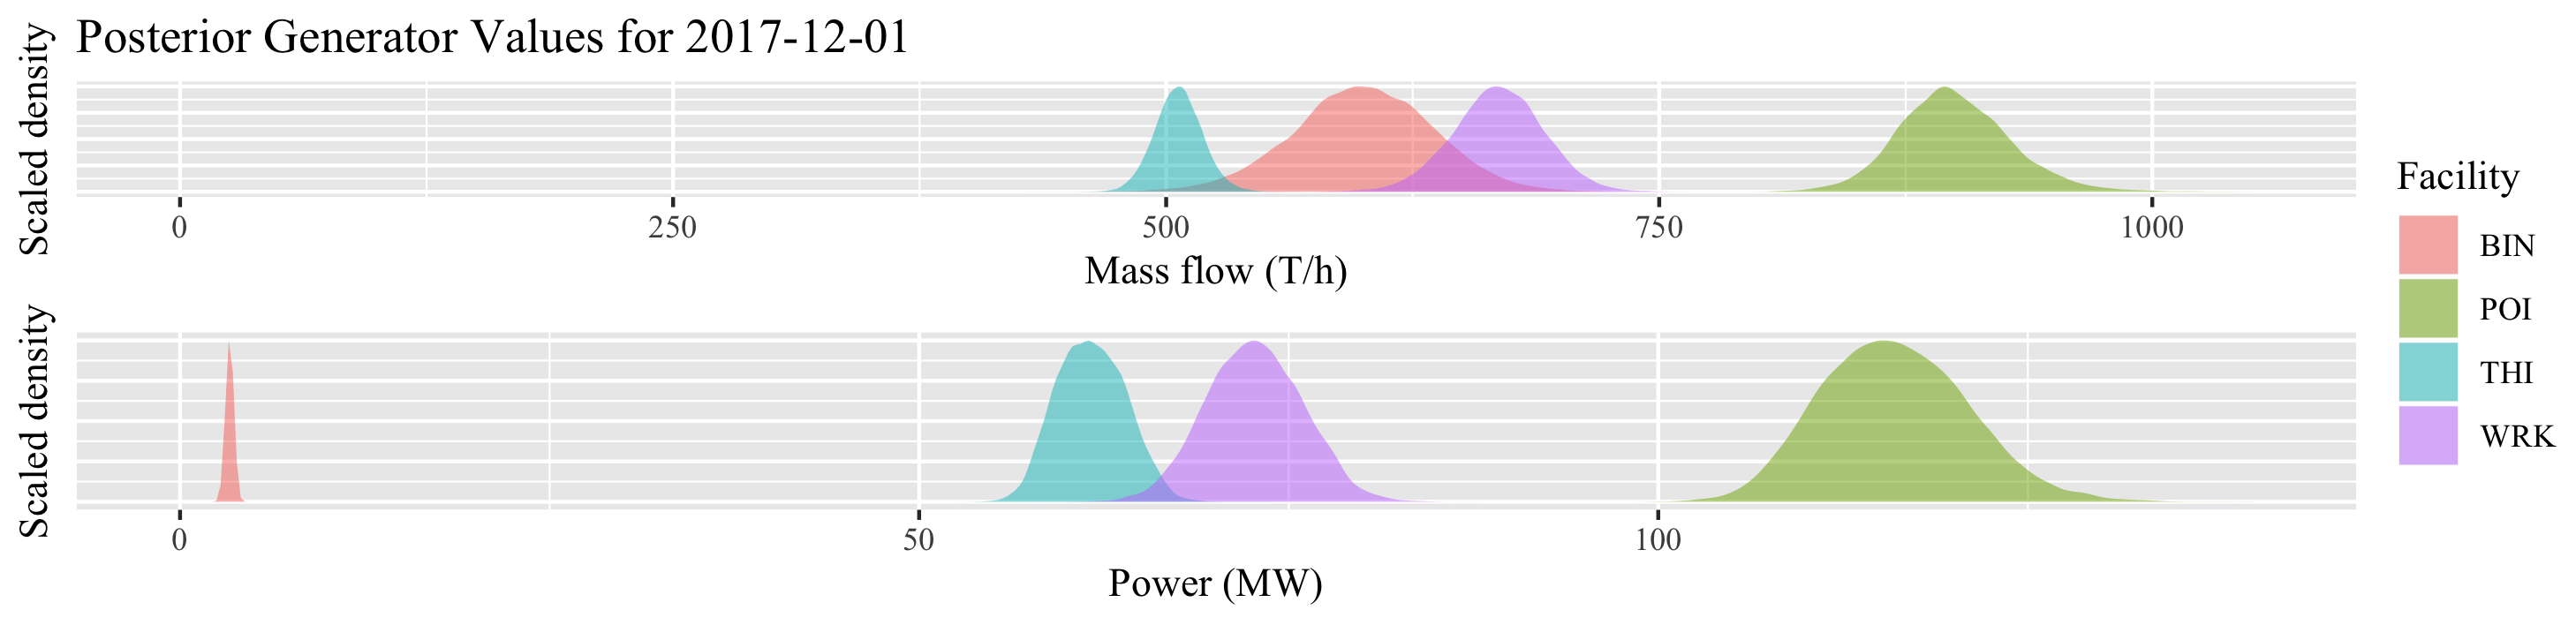
\includegraphics[width=\linewidth]{media/gens}
  \captionof{figure}{Estimates for mass flow and power generation, accounting for uncertainties for the steam/power conversion factor.}
  \label{fig:gens}
\end{figure}

%%%%%%%%%%%%%%%%%%%%%%%%%%%%%%%%%
\section{Conclusions}
In this report, we show a hierarchical regression model and a directed network with uncertainty can be implemented in a single Bayesian model to estimate the true state of a geothermal surface network. Our model includes estimates of errors in both the steady-state properties of the network such as flows, and in the regression parameters such as production decline in the wells.

Our model addresses two needs:
\begin{enumerate}
\item Produce production curves with uncertainty so the operator can track well declines and see how mass flow changes with well-head pressure.
\item Make forecasts, both short-term and long-term to see how the field changes over time.
\end{enumerate}
We also compare our posterior beliefs of the network against constraints set by the field's operators, and find that our simulation is able to probabilistically verify whether those constraints are violated in a given network configuration, as long as we have sufficient test data or PI data about the wells feeding a facility.

Despite CEL and Grant \& Bixley using an elliptic or otherwise curved model in their regression \cite{Grant:2011}, we do not find significant evidence that the data would be better suited by a non-linear model. We are also able to incorporate all historical test data into a regression model for the production curves, giving good parameter estimates for a temporal decline model and better robustness compared with CEL's current methods.

When the goal is to make mass flow forecasts, a production curve can give comparable precision to time-series analysis. However, using the production curve also creates extra error if the well-head pressure is incorrect, or if there is insufficient data such as PI logs recorded near the operational well-head pressure. Incorporating PI data into the regression also improves our forecasting accuracy because the PI data is recent. The tradeoff is that adding PI data decreases precision in the regression parameters because the concentrated data forces the regression to pass through a point. This may be undesirable if the parameters representing mass flow decline with pressure or time are more important than forecasts.

All of the figures presented in this report as also available as interactive HTML widgets, allowing the operator to filter down to individual wells or subsets. Model operation is designed to be non-technical, so that any existing operator can interpret uncertainty and credible intervals just as they would with the current Excel model. To make changes, we provide a configuration spreadsheet where the well/flash-plant and flash-plant/generator connectivity is specified, either as the output of an external third-party optimisation algorithm \cite{Fox:2018} or as part of scenario analysis. This spreadsheet is also where constants such as enthalpy are specified.

%\todo{Note about performance and use cases -- should it be used}

%%%%%%%%%%%%%%%%%%%%%%%%%%%%%%%%%
\section{Further Development}
There are many opportunities to expand on the utility of this work.

\subsection{Enthalpy Prediction}
Currently we fix enthalpy as a known constant by using the most recent enthalpy as calculated by CEL in their spreadsheets. We do this because enthalpy does not vary as much and is not as critical as mass flow. However, better uncertainty would be gained by regressing enthalpy with well-head pressure and especially time.

\subsection{Direct Data Integration}
In this work, all data was obtained through Excel workbooks, even though some of it was originally stored in a PI system. Direct integration with the PI database would have benefits:

\begin{enumerate}
\item Automatic daily updates can track changes in trend live within 24 hours. Our system is designed to deliver information within minutes, but this is only relevant if it is not bottlenecked by data access.
\item When available, data from the PI system is superior because it is automatically recorded once a day, and is more recent. There were issues with interpreting variable names and encoding that meant we ignored some data, but access to a documented PI database would allow us to incorporate more variables.
\end{enumerate}

\subsection{Data Integration With Other Models}
Enthalpies are important because they affect the mass proportions exiting the flash plant. We use the most recent recorded enthalpy for each well, and do a probabilistic imputation for wells with unknown enthalpies. Taking simulation results from a wellbore simulator such as TOUGH2 would avoid the uncertainty associated with imputation, and may also give us more up-to-date enthalpies.

\subsection{Time Series}
In our implementation of well declines, we treat measurements independently with respect to time. However, measurements are almost never truly independent and are often auto-correlated with previous measurements. Our JAGS model includes promising experiments for autoregression and weighted moving-average methods (Figure \ref{fig:ts_experiment}), but they cannot be applied for all the wells right now because they require evenly spaced data such as PI data, rather than irregular test data.

We would also be interested to compare the performance of a standalone AR(1) forecast without any production curves. The downsides include having no estimate for the parameterisation of mass flow, and not having flow meters for all the wells. A proof of concept may provide motivation to install more flow meters.

\subsection{Prior Specification}
More prior specifications for parameters will add extra educated bias to our model, helping with variance reduction and requiring less data for parameters that are expensive to measure. Priors can be added to the hierarchical parameters on the regression coefficients, which are currently non-informative. For instance, if we knew an overall production decline rate and variance in decline across the field.

\subsection{Hierarchical Model Resolution}
Partitioning of network components by manufacturer's specifications or age/generation will improve the hierarchical model. We currently treat all wells or flash plants as coming from the same family of facilities. However, we know the Wairakei geothermal field was built in a series of stages and that some facilities are more similar than others. Each family of facility should have its own hierarchical model, reducing variance in the hyper-parameters.

\newpage
\bibliography{bibliography} 

\newpage
\begin{appendices}
\section{Time Series Comparison}
\begin{figure}[H]
  \centering
  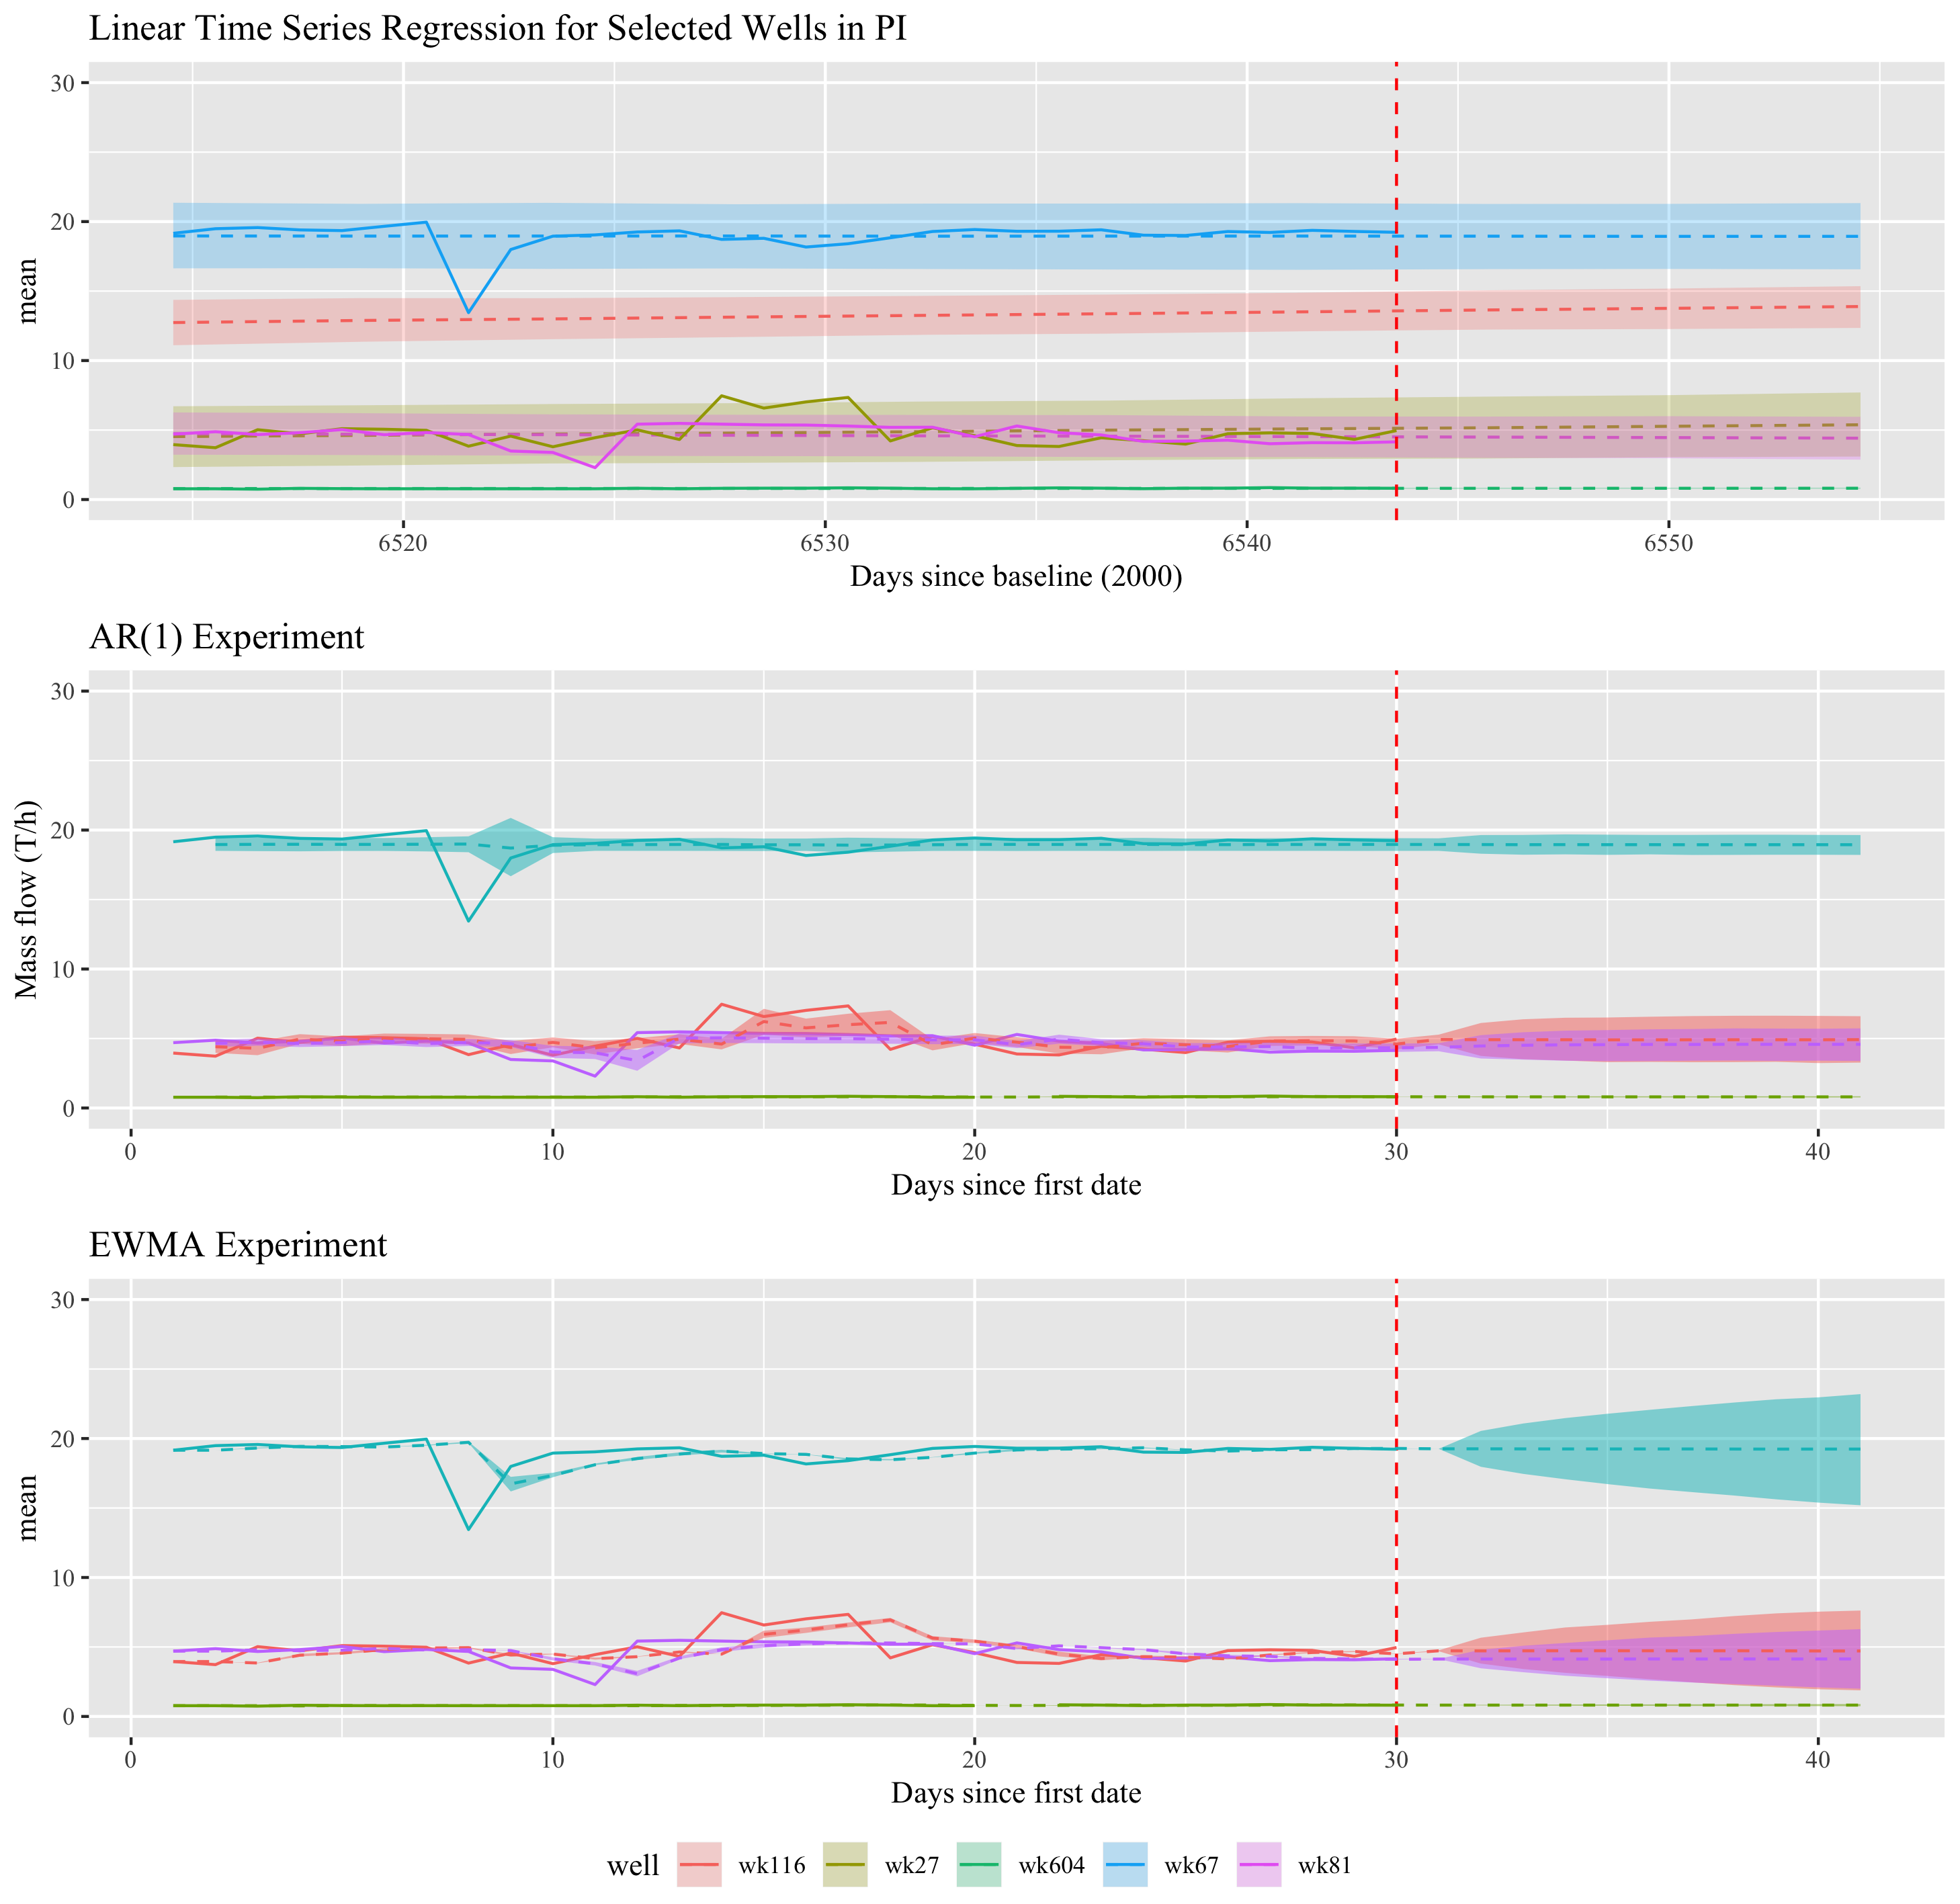
\includegraphics[width=\linewidth]{media/ts_experiment}
  \captionof{figure}{Time-series techniques on data from the PI database. We use the linear time series regression (top) for its robustness to systematic changes in operation, which can cause the other regressions to display unstable behaviour. Auto-regression and exponentially-weighted moving average techniques both have their strengths and weaknesses.}
  \label{fig:ts_experiment}
\end{figure}

\newpage
\section{Regression Diagnostics}
\begin{figure}[H]
  \centering
  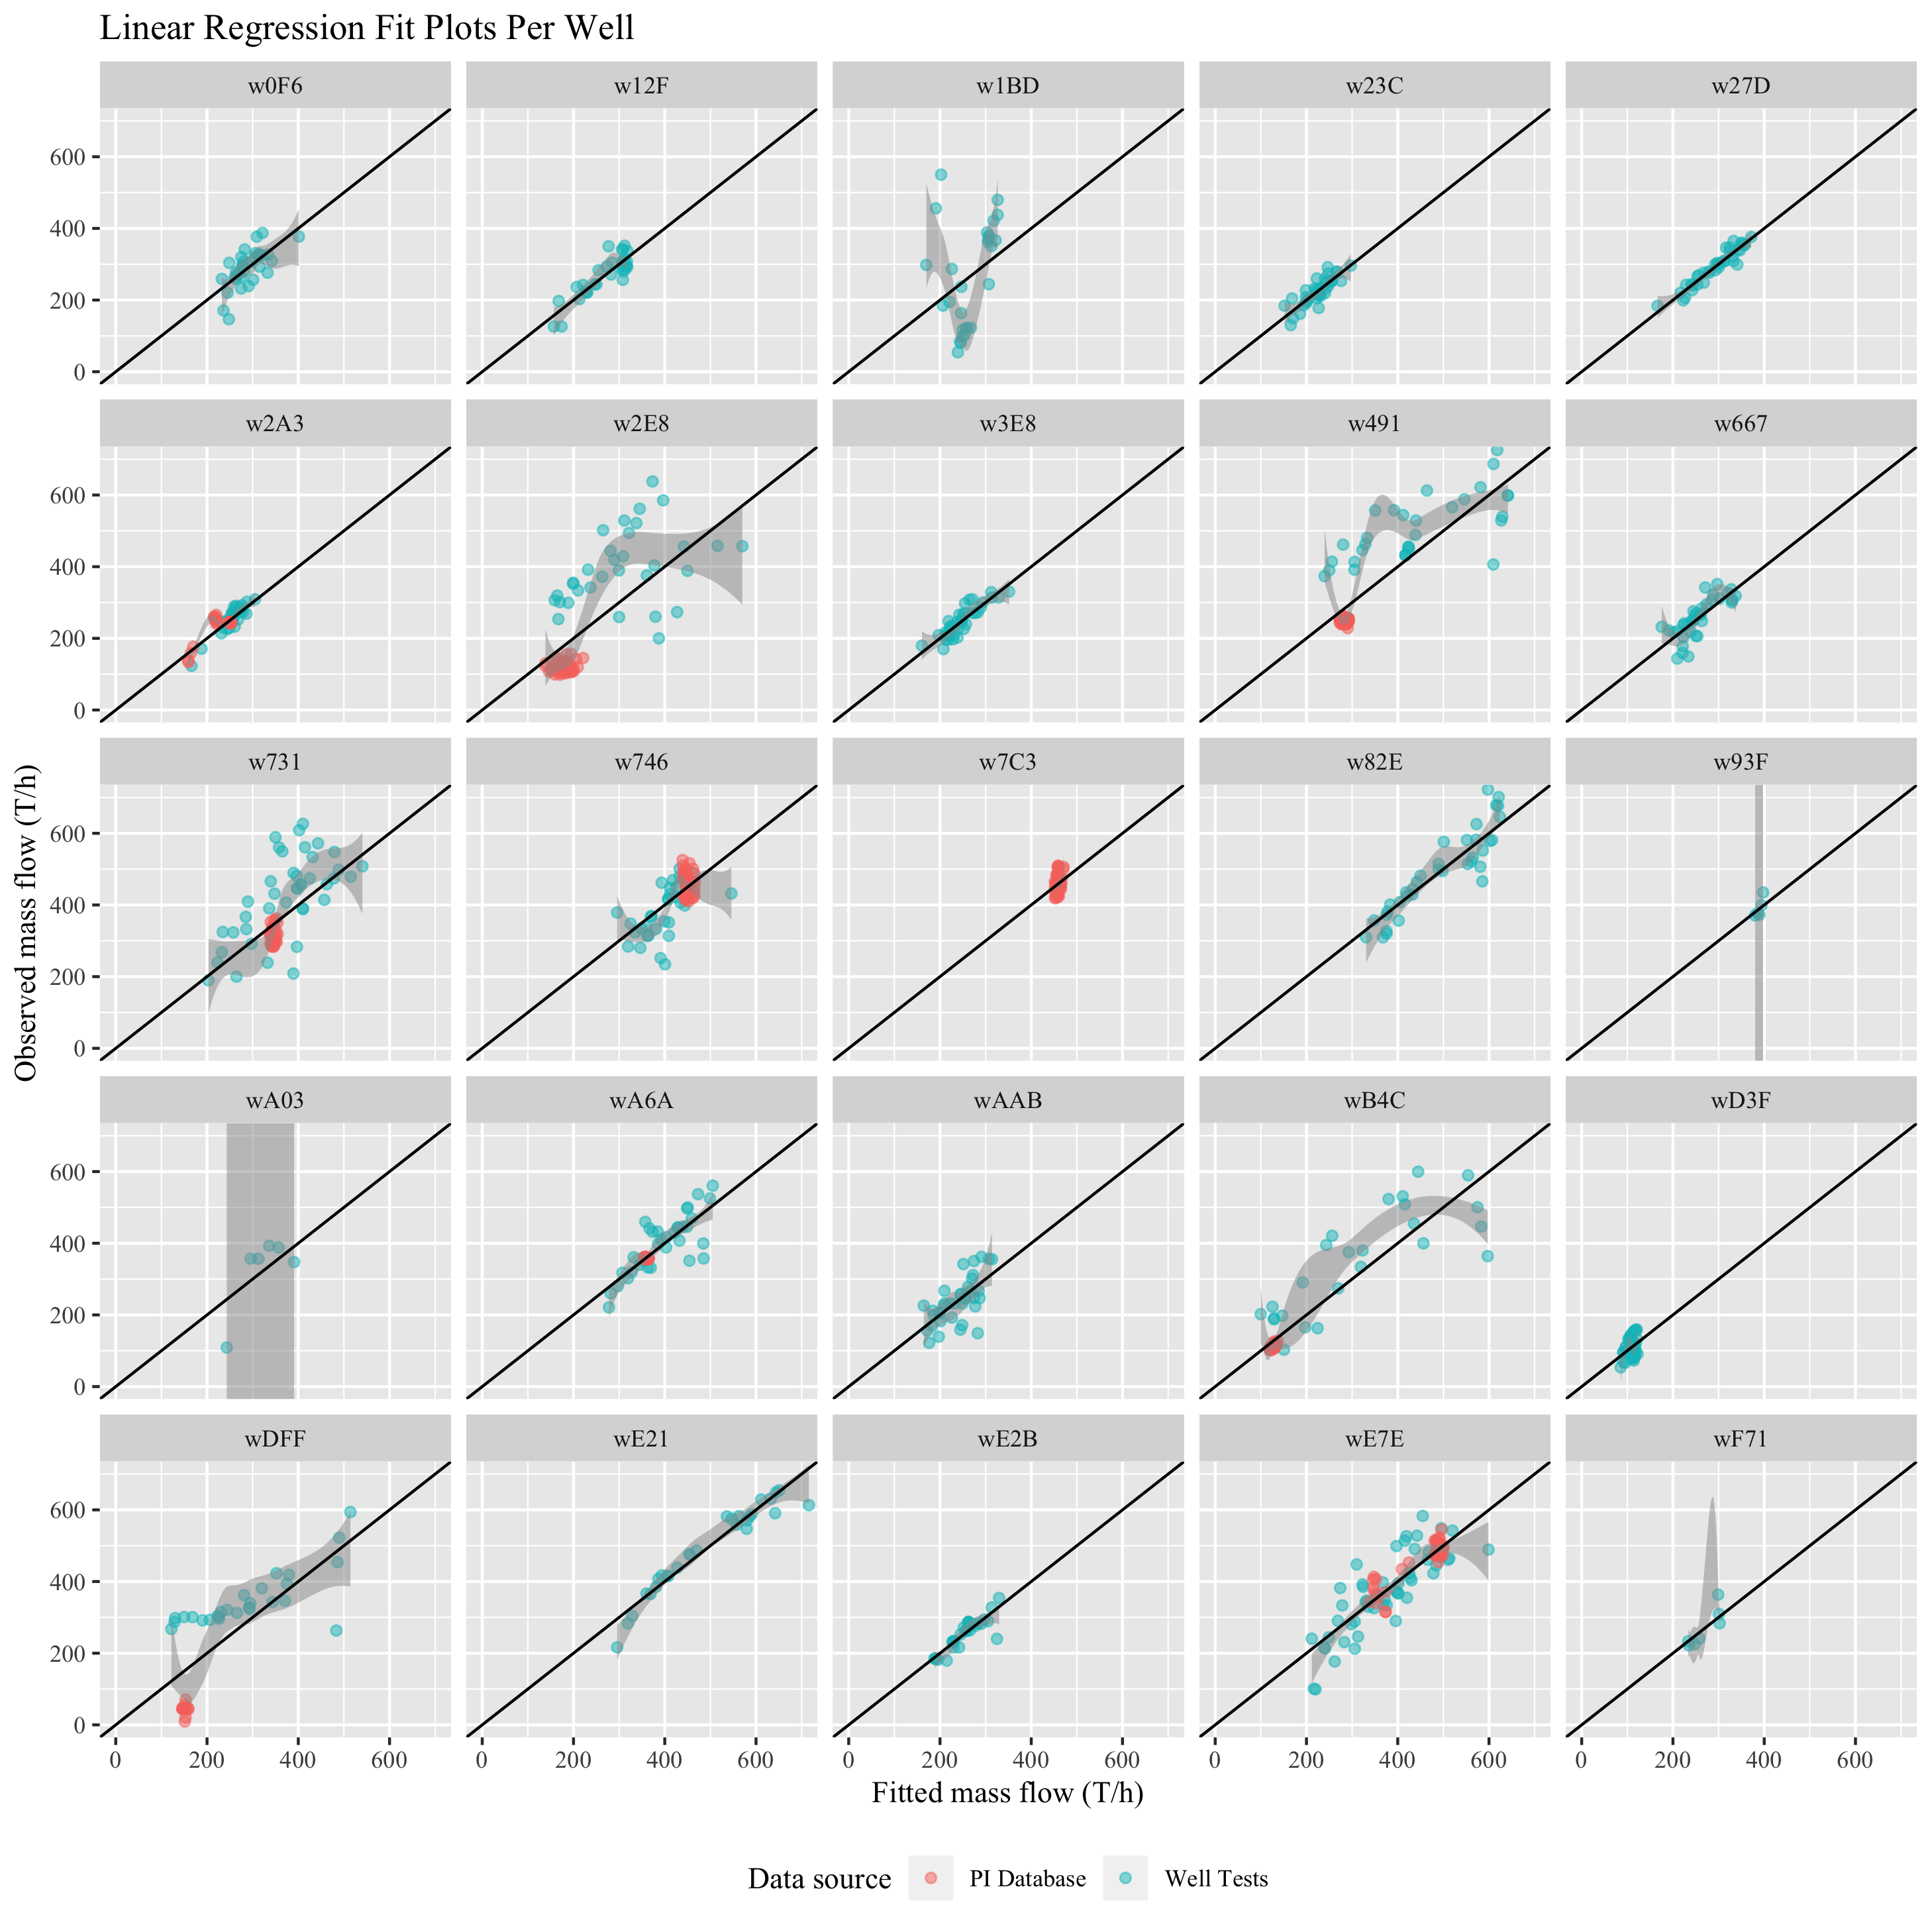
\includegraphics[width=\linewidth]{media/observed}
  \captionof{figure}{95\% LOESS smoothing shaded in, and $y=x$ line in black. Observed vs fitted plots per well show good fits for some wells and slight curvature in others. However, the curvature is not common and is likely due to random variation. Only wells with non-singular well-head pressures shown.}
  \label{fig:observed}
\end{figure}

\begin{figure}[H]
  \centering
  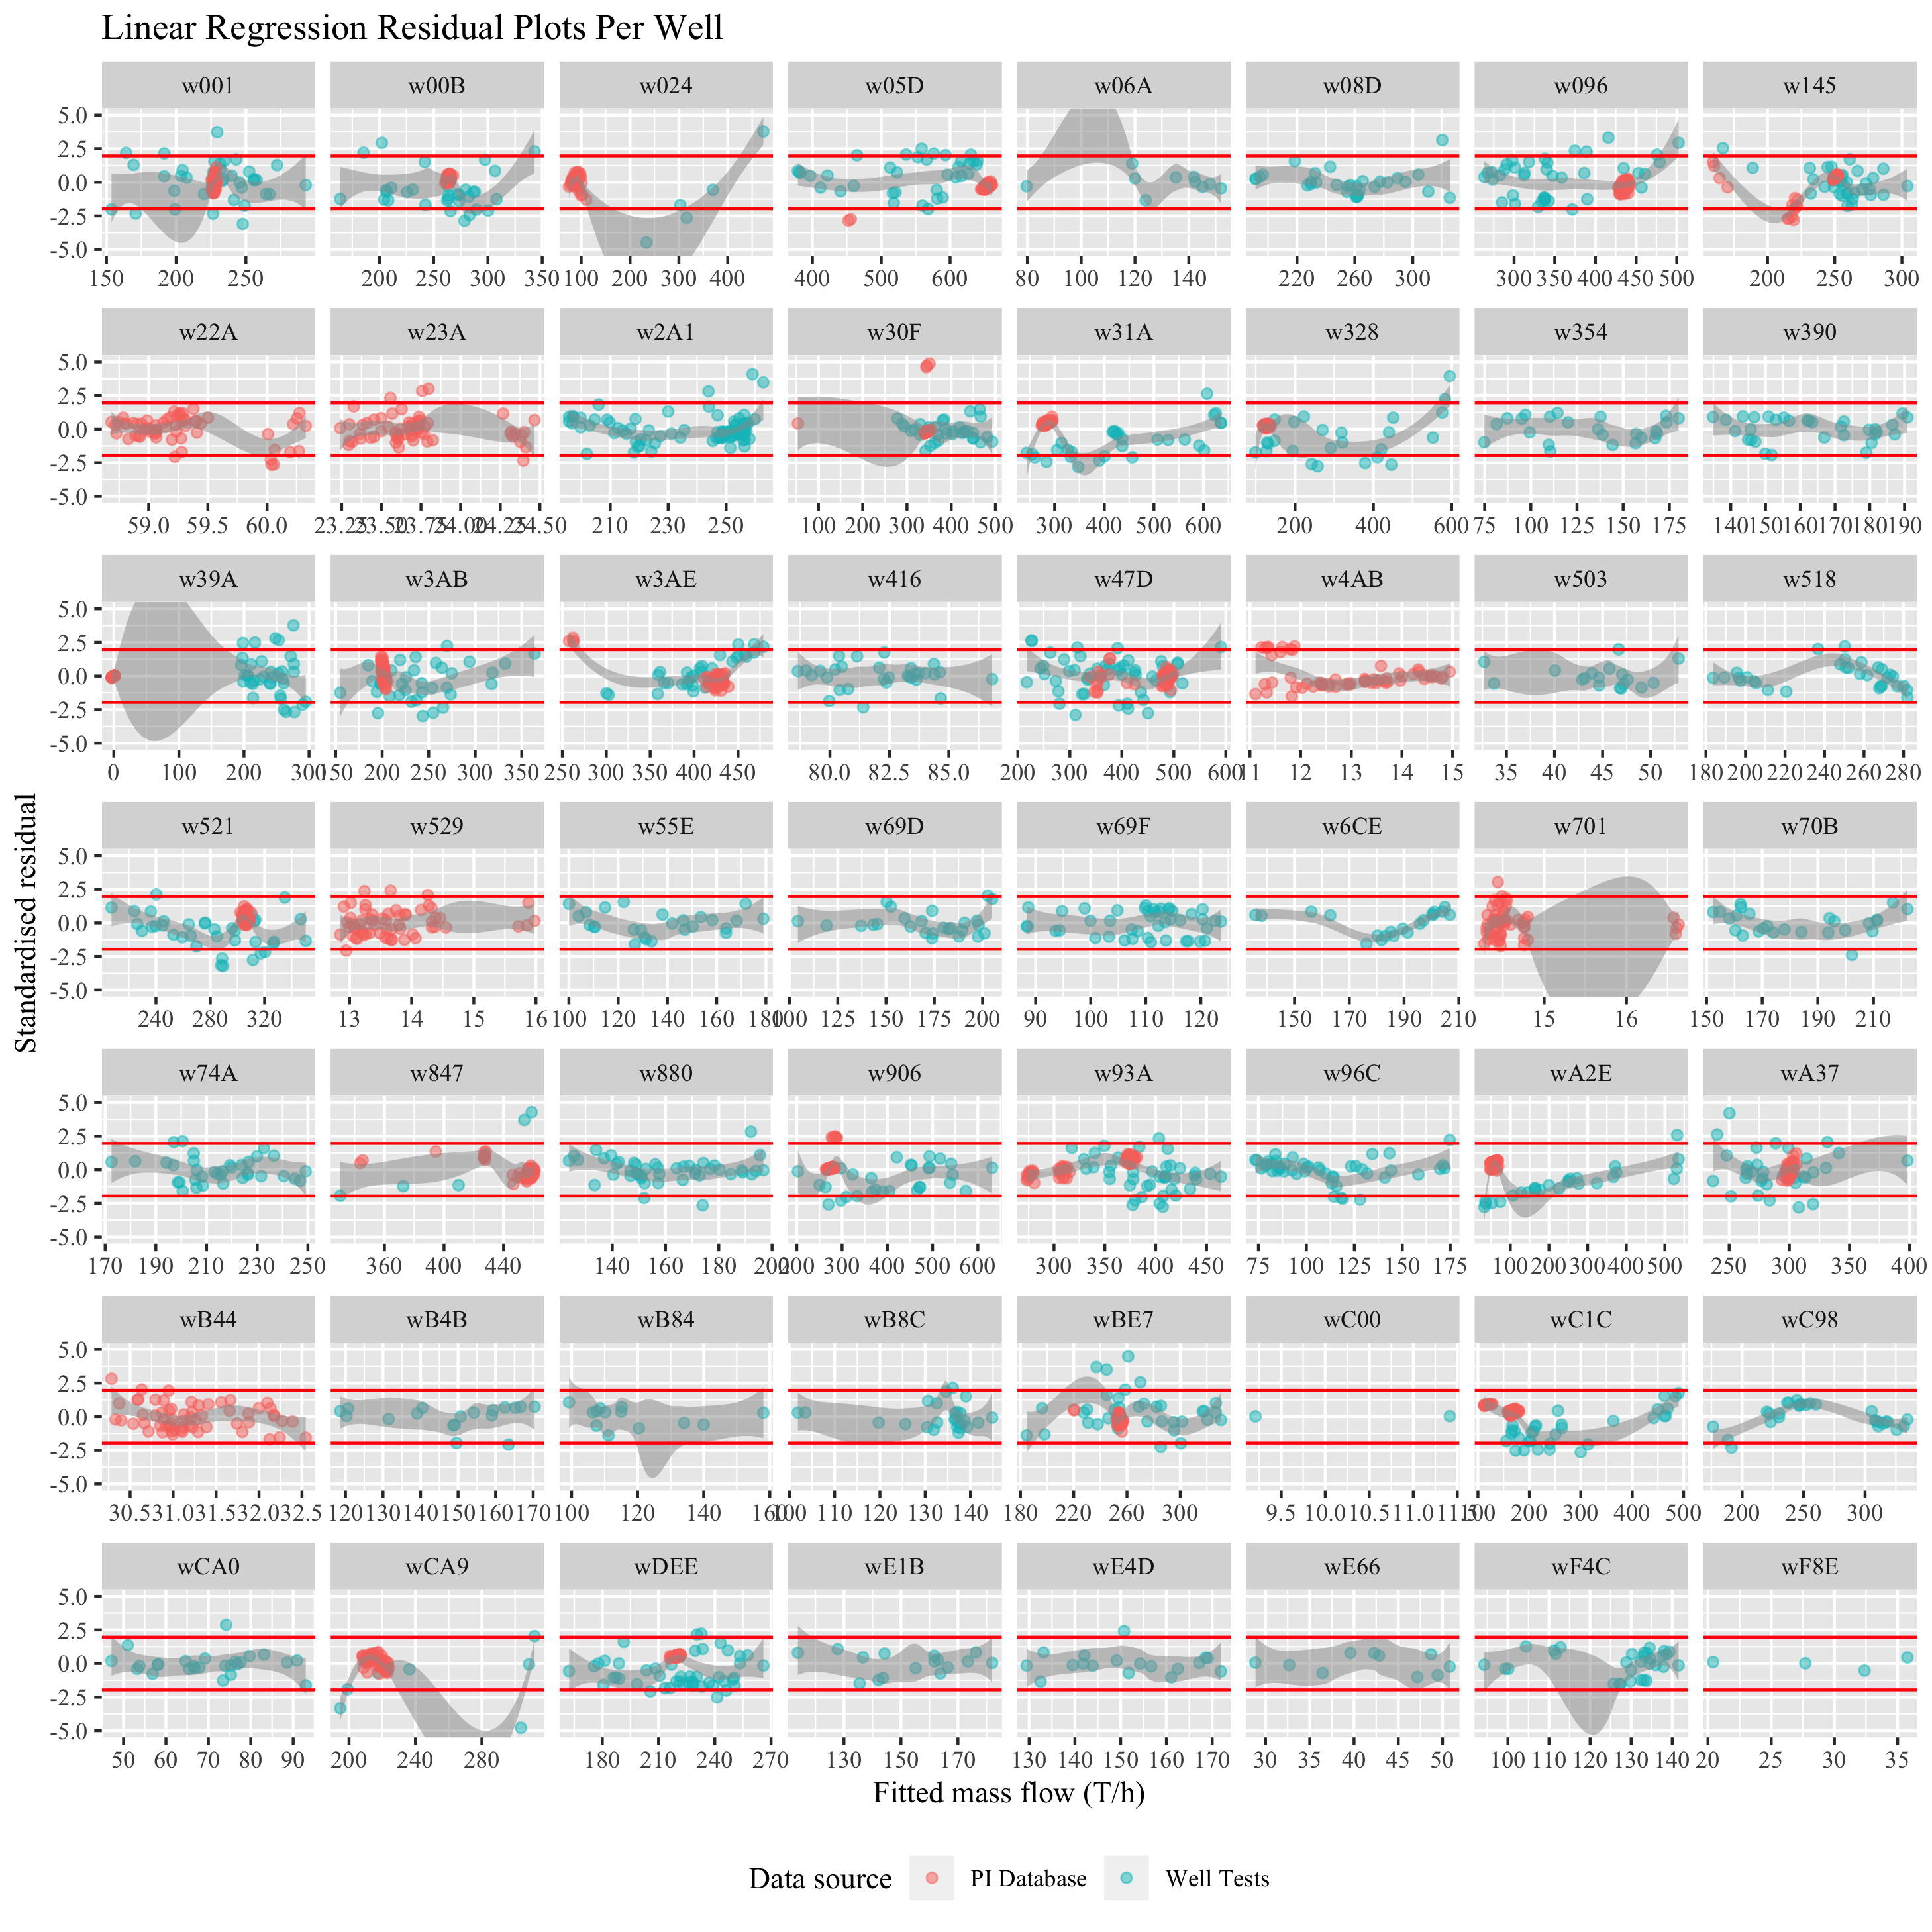
\includegraphics[width=\linewidth]{media/stdres}
  \captionof{figure}{95\% LOESS smoothing shaded in. Some of the wells show curvature but not enough to make the DIC favour a quadratic model. Only wells with non-singular well-head pressures shown.}
  \label{fig:stdres}
\end{figure}

\newpage
\section{All Well Declines}
% latex table generated in R 3.4.2 by xtable 1.8-2 package
% Wed Sep 19 14:29:23 2018
\begin{table}[ht]
\centering
\begingroup\fontsize{11pt}{11pt}\selectfont
\begin{tabular}{lrrrr}
  \hline
well & Mean & Lower 2.5\% & Upper 97.5\% & n \\ 
  \hline
w0F6 & -0.046 & -0.067 & -0.025 &   33 \\ 
  w12F & -0.019 & -0.035 & -0.002 &   32 \\ 
  w1BD & 0.021 & -0.008 & 0.049 &   28 \\ 
  w23C & -0.024 & -0.032 & -0.016 &   39 \\ 
  w27D & -0.024 & -0.031 & -0.017 &   37 \\ 
  w2A3 & -0.015 & -0.021 & -0.010 &   95 \\ 
  w2E8 & -0.214 & -0.276 & -0.154 &   82 \\ 
  w3E8 & -0.067 & -0.079 & -0.055 &   38 \\ 
  w491 & -0.302 & -0.354 & -0.247 &   92 \\ 
  w4B1 & 0.007 & -0.002 & 0.017 &   61 \\ 
  w5BC & 0.000 & -0.010 & 0.013 &   61 \\ 
  w667 & -0.062 & -0.082 & -0.044 &   37 \\ 
  w680 & -0.053 & -0.113 & 0.000 &   58 \\ 
  w731 & -0.161 & -0.203 & -0.120 &  102 \\ 
  w746 & 0.005 & -0.014 & 0.024 &   91 \\ 
  w793 & -0.015 & -0.039 & 0.007 &   61 \\ 
  w7C3 & 0.001 & -0.152 & 0.163 &   61 \\ 
  w7FA & -0.031 & -0.037 & -0.026 &   61 \\ 
  w82E & -0.144 & -0.177 & -0.109 &   36 \\ 
  w93F & -0.108 & -0.287 & 0.063 &    5 \\ 
  w9A0 & -0.035 & -0.084 & -0.003 &   61 \\ 
  wA03 & -0.076 & -0.242 & 0.085 &    6 \\ 
  wA6A & -0.150 & -0.172 & -0.129 &   91 \\ 
  wA99 & -0.046 & -0.062 & -0.029 &   61 \\ 
  wAAB & -0.053 & -0.073 & -0.032 &   37 \\ 
  wB4C & -0.141 & -0.192 & -0.090 &   86 \\ 
  wB8D & -0.021 & -0.038 & -0.003 &   61 \\ 
  wBA2 & -0.005 & -0.042 & 0.040 &   61 \\ 
  wCAA & -0.011 & -0.031 & 0.008 &   61 \\ 
  wD3F & 0.001 & -0.005 & 0.007 &   44 \\ 
  wDFF & -0.214 & -0.288 & -0.138 &   42 \\ 
  wE21 & -0.126 & -0.158 & -0.093 &   29 \\ 
  wE2B & -0.063 & -0.087 & -0.039 &   31 \\ 
  wE7E & -0.062 & -0.074 & -0.049 &  113 \\ 
  wF71 & -0.159 & -0.321 & 0.003 &    7 \\ 
   \hline
\end{tabular}
\endgroup
\caption{Credible intervals for $\beta_\text{date}$ in units T/h/d.} 
\label{tab:beta_date_all}
\end{table}


\newpage
\section{Flash Plant Data Sources} \label{sec:fpdata}
% latex table generated in R 3.4.2 by xtable 1.8-2 package
% Fri Sep 21 13:38:25 2018
\begin{table}[H]
\centering
\begin{tabular}{rlrrrr}
  \hline
 & facility & mean & sd & n\_test & n\_pi \\ 
  \hline
1 & wC98 & 323.42 & 45.70 &  28 &   0 \\ 
  2 & w3AE & 393.84 & 16.31 &  34 &  30 \\ 
  3 & w096 & 419.71 & 15.16 &  41 &  30 \\ 
  4 & w30F & 334.66 & 14.26 &  34 &  30 \\ 
  5 & w69F & 107.26 & 8.39 &  44 &   0 \\ 
  6 & w47D & 375.03 & 8.38 &  52 &  30 \\ 
  7 & w145 & 221.51 & 3.24 &  34 &  30 \\ 
  8 & wBD9 & 14.24 & 1.00 &   0 &  30 \\ 
  9 & w529 & 13.68 & 0.63 &   0 &  30 \\ 
  10 & w701 & 15.00 & 0.12 &   0 &  30 \\ 
   \hline
\end{tabular}
\caption{Data methods feeding flash plant fp24} 
\label{tab:well_summaries_fp14}
\end{table}

% latex table generated in R 3.4.2 by xtable 1.8-2 package
% Mon Sep 17 20:29:28 2018
\begin{table}[H]
\centering
\begin{tabular}{rlrrrrlll}
  \hline
 & facility & mean & sd & n\_test & n\_pi & use.test & use.pi & production.curve \\ 
  \hline
1 & wF71 & 239.82 & 22.51 &   7 &   0 & Test data & No PI data & Production curve \\ 
  2 & wDFF & 144.01 & 20.60 &  27 &  15 & Test data & PI data & Production curve \\ 
  3 & w2E8 & 197.52 & 13.25 &  32 &  50 & Test data & PI data & Production curve \\ 
  4 & w491 & 273.42 & 8.75 &  31 &  61 & Test data & PI data & Production curve \\ 
  5 & w731 & 340.68 & 8.13 &  41 &  61 & Test data & PI data & Production curve \\ 
  6 & wB4C & 119.93 & 7.52 &  25 &  61 & Test data & PI data & Production curve \\ 
  7 & w9BD & 15.61 & 0.61 &   0 &   0 & No test data & No PI data & Time series \\ 
  8 & wBA2 & 45.83 & 0.46 &   0 &  61 & No test data & PI data & Production curve \\ 
  9 & w793 & 197.89 & 0.35 &   0 &  61 & No test data & PI data & Production curve \\ 
  10 & wCAA & 59.86 & 0.29 &   0 &  61 & No test data & PI data & Production curve \\ 
  11 & w5BC & 22.67 & 0.29 &   0 &  61 & No test data & PI data & Production curve \\ 
  12 & wA99 & 30.25 & 0.17 &   0 &  61 & No test data & PI data & Production curve \\ 
  13 & w7FA & 58.46 & 0.17 &   0 &  61 & No test data & PI data & Production curve \\ 
  14 & wB8D & 22.96 & 0.14 &   0 &  61 & No test data & PI data & Production curve \\ 
   \hline
\end{tabular}
\caption{Data methods feeding flash plant fp62} 
\label{tab:well_summaries_fp15}
\end{table}

% latex table generated in R 3.4.2 by xtable 1.8-2 package
% Fri Sep 21 13:38:25 2018
\begin{table}[H]
\centering
\begin{tabular}{rlrrrr}
  \hline
 & facility & mean & sd & n\_test & n\_pi \\ 
  \hline
1 & w906 & 324.11 & 16.73 &  29 &  30 \\ 
  2 & w05D & 633.00 & 9.80 &  36 &  30 \\ 
  3 & w024 & 86.32 & 6.60 &   6 &  30 \\ 
  4 & wA37 & 295.99 & 4.86 &  33 &  30 \\ 
  5 & w00B & 269.63 & 4.63 &  32 &  30 \\ 
  6 & wBE7 & 250.25 & 4.57 &  37 &  30 \\ 
  7 & w847 & 461.02 & 4.09 &   5 &  30 \\ 
  8 & w3AB & 198.62 & 3.37 &  38 &  30 \\ 
  9 & w521 & 309.07 & 3.28 &  37 &  30 \\ 
  10 & w001 & 226.67 & 2.44 &  39 &  30 \\ 
   \hline
\end{tabular}
\caption{Data methods feeding flash plant fp28} 
\label{tab:well_summaries_fp16}
\end{table}


\newpage
\section{JAGS Model} \label{sec:jagscode}
The following model is loaded as a text string into the RJAGS package. Not listed is the data, pre-processing code and post-processing of the results. This code also includes two extra time-series models that were not used for outputs. (Pre-/post-processing source code available on the author's Github)

\lstinputlisting[language=R, firstline=2]{src/model.txt}

\end{appendices}
\end{document}